\Opensolutionfile{ans}[ans/ansCD2D2-6.0]
% \section{BẤT PHƯƠNG TRÌNH MŨ VÀ BẤT PHƯƠNG TRÌNH LOGARIT}
\begin{center}
	\textbf{CHUYÊN ĐỀ 3: Bất phương trình mũ}
\end{center}
\subsection{Kiến thức sách giáo khoa cần cần nắm}
Ta có thể dùng các phương pháp biến đổi như phương trình mũ và các công thức sau:
\begin{itemize}
	\item[$\bullet$] Nếu $a>1$ thì: $a^{f(x)}>a^{g(x)}\Leftrightarrow f(x)>g(x)$ và $a^{f(x)}\geq a^{g(x)}\Leftrightarrow f(x)\geq g(x)$.
	\item[$\bullet$] Nếu $0<a<1$ thì: $a^{f(x)}>a^{g(x)}\Leftrightarrow f(x)<g(x)$ và $a^{f(x)}\geq a^{g(x)}\Leftrightarrow f(x)\leq g(x)$.
\end{itemize}
Tổng quát ta có:
\begin{itemize}
	\item[$\bullet$] $a^{f(x)}>a^{g(x)}\Leftrightarrow\heva{&a>0\\&(a-1)\cdot [f(x)-g(x)]>0.}$
	\item[$\bullet$] $a^{f(x)}\geq a^{g(x)}\Leftrightarrow\heva{&a>0\\&(a-1)\cdot [f(x)-g(x)]\geq 0.}$
\end{itemize}
\subsection{Phân loại và phương pháp giải bài tập}
\begin{dang}{Phương pháp đưa về cơ số và logarit hóa}
	Phương pháp:
	\begin{itemize}
		\item[$\bullet$] Nếu $a>1$ thì: $a^{f(x)}>a^{g(x)}\Leftrightarrow f(x)>g(x)$ và $a^{f(x)}\geq a^{g(x)}\Leftrightarrow f(x)\geq g(x)$.
		\item[$\bullet$] Nếu $0<a<1$ thì: $a^{f(x)}>a^{g(x)}\Leftrightarrow f(x)<g(x)$ và $a^{f(x)}\geq a^{g(x)}\Leftrightarrow f(x)\leq g(x)$.
	\end{itemize}
\end{dang}
\subsubsection{Các ví dụ}
\setcounter{vd}{0}
\begin{vd}%[2D2B6-2]%Ví dụ 1.
	Tìm tập nghiệm của bất phương trình $\left(\dfrac{3}{4}\right)^{2x-1}\leq\left(\dfrac{3}{4}\right)^{2-x}$.
	\loigiai{
		Ta có $\left(\dfrac{3}{4}\right)^{2x-1}\leq\left(\dfrac{3}{4}\right)^{2-x}\Leftrightarrow 2x-1\geq 2-x\Leftrightarrow x\geq 1$.}
\end{vd}
\begin{vd}%[2D2B6-2]%Ví dụ 2.
	Giải bất phương trình $2^{-x^2+3x}<4$.
	\loigiai{
		Do $2>1$ nên $2^{-x^2+3x}<4\Leftrightarrow-x^2+3x<2\Leftrightarrow\hoac{&x<1\\&x>2.}$ \\
		Vậy tập nghiệm của bất phương trình là $(-\infty;1)\cup(2;+\infty)$.}
\end{vd}
\begin{vd}%[2D2B6-2]%Ví dụ 3.
	Tìm nghiệm của bất phương trình $2^{x^2+3x-2}\geq\dfrac{1}{4}$.
	\loigiai{
		Ta có $2^{x^2+3x-2}\geq\dfrac{1}{4}\Leftrightarrow 2^{x^2+3x-2}\geq 2^{-2}\Leftrightarrow x^2+3x-2\geq-2$ \\
		$ \Leftrightarrow x^2+3x\geq 0\Leftrightarrow\hoac{&x\geq 0\\&x\leq-3.} $}
\end{vd}
\begin{vd}%[2D2B6-2]%Ví dụ 4.
	Bất phương trình $2^{x^2-3x+4}\leq\left(\dfrac{1}{2}\right)^{2x-10}$ có bao nhiêu nghiệm nguyên dương?
	\loigiai{
		Bất phương trình tương đương với
		\allowdisplaybreaks
		\begin{eqnarray*}
			& & 2^{x^2-3x+4}\leq 2^{10-2x}\Leftrightarrow x^2-3x+4\leq 10-2x\\
			&\Leftrightarrow & x^2-x-6\leq 0 \Leftrightarrow-2\leq x\leq 3.
		\end{eqnarray*}
		Do $x>0$ nên $0<x\leq 3$.\\
		Mà $x\in\mathbb{Z}^+$ nên $x\in\{1;2;3\}$. Vậy có $3$ giá trị nguyên dương thỏa mãn yêu cầu bài toán.}
\end{vd}
\begin{vd}%[2D2B6-2]%Ví dụ 5.
	Tìm nghiệm của bất phương trình: $\left(\dfrac{3}{5}\right)^{x^2-2x-1}\geq\left(\dfrac{25}{9}\right)^{2x-1}$.
	\loigiai{
		Bất phương trình $\Leftrightarrow\left(\dfrac{3}{5}\right)^{x^2-2x-1}\geq\left(\dfrac{3}{5}\right)^{-4x+2}\Leftrightarrow x^2+2x-3\leq 0\Leftrightarrow -3\leq x\leq 1$.}
\end{vd}
\begin{vd}%[2D2B6-2]%Ví dụ 6.
	Tìm nghiệm của bất phương trình: $(2-\sqrt{3})^{x^2-3x}>(2+\sqrt{3})^2$.
	\loigiai{
		Có $(2+\sqrt{3})(2-\sqrt{3})=1\Rightarrow 2+\sqrt{3}=\dfrac{1}{2-\sqrt{3}}=(2-\sqrt{3})^{-1}$.\\
		Bất phương trình $\Leftrightarrow(2-\sqrt{3})^{x^2-3x}>(2-\sqrt{3})^{-2}\Leftrightarrow x^2-3x+2<0\Leftrightarrow 1<x<2$.}
\end{vd}
\begin{vd}%[2D2B6-2]%Ví dụ 7.
	Tìm tập nghiệm của bất phương trình $5^{x+1}-\dfrac{1}{5}>0$.
	\loigiai{
		Ta có: $5^{x+1}-\dfrac{1}{5}>0\Leftrightarrow 5^{x+1}-5^{-1}>0\Leftrightarrow x+1 >-1\Leftrightarrow x >-2\Rightarrow S=(-2;+\infty)$.}
\end{vd}
\begin{vd}%[2D2B6-4]%Ví dụ 8.
	Bất phương trình $2^{x^2}\cdot 3^x<1$ có bao nhiêu nghiệm nguyên?
	\loigiai{
		Ta có $2^{x^2}\cdot 3^x<1\Leftrightarrow x^2+x\cdot\log_23<0\Leftrightarrow x(x+\log_23)<0\Leftrightarrow -\log_23<x<0$.\\
		Suy ra bất phương trình có một nghiệm nguyên $x=-1$.}
\end{vd}
\subsubsection{Câu hỏi trắc nghiệm}
\begin{ex}%[2D2Y1-3]%Câu 1.
	Cho $(2-\sqrt{3})^m>(2-\sqrt{3})^n\quad(m,n\in\mathbb{Z})$. Khẳng định nào sau đây là khẳng định đúng?
	\choice
	{$m>n$}
	{\True $m<n$}
	{$m=n$}
	{$m\geq n$}
	\loigiai{
		Ta có $0<2-\sqrt{3}<1\Rightarrow(2-\sqrt{3})^m>(2-\sqrt{3})^n\Rightarrow m<n$.}
\end{ex}
\begin{ex}%[2D2B6-1]%Câu 2.
	Cho $0<a<1$. Khẳng định nào dưới đây là đúng?
	\choice
	{$a^x>1\Leftrightarrow x\geq 0$}
	{$a^x>1\Leftrightarrow x>0$}
	{\True $a^x>1\Leftrightarrow x<0$}
	{$a^x>1\Leftrightarrow 0<x<1$}
	\loigiai{
		Do $0<a<1$ nên $a^x>1\Leftrightarrow a^x>a^{\circ}\Leftrightarrow x<0$.}
\end{ex}
\begin{ex}%[2D2Y6-2]%Câu 3.
	Nghiệm của bất phương trình $3^{2x+1}>3^{3-x}$ là 
	\choice
	{$x>\dfrac{3}{2}$}
	{$x<\dfrac{2}{3}$}
	{$x >-\dfrac{2}{3}$}
	{\True $x>\dfrac{2}{3}$}
	\loigiai{
		$3^{2x+1}>3^{3-x}\Leftrightarrow 2x+1>3-x\Leftrightarrow x>\dfrac{2}{3}$.}
\end{ex}
\begin{ex}%[2D2B1-3]%Câu 4.
	Cho $\alpha$, $\beta$ là hai số thực. Khẳng định nào sau đây là khẳng định đúng?
	\choice
	{$\left(\dfrac{2}{\mathrm{e}}\right)^{\alpha}>\left(\dfrac{2}{\mathrm{e}}\right)^{\beta}\Leftrightarrow\alpha,\beta$ là hai số thực luôn luôn dương}
	{$\left(\dfrac{2}{\mathrm{e}}\right)^{\alpha}>\left(\dfrac{2}{\mathrm{e}}\right)^{\beta}\Leftrightarrow\alpha>\beta$}
	{$\left(\dfrac{2}{\mathrm{e}}\right)^{\alpha}>\left(\dfrac{2}{\mathrm{e}}\right)^{\beta}\Leftrightarrow\alpha,\beta$ là hai số thực không âm}
	{\True $\left(\dfrac{2}{\mathrm{e}}\right)^{\alpha}>\left(\dfrac{2}{\mathrm{e}}\right)^{\beta}\Leftrightarrow\alpha<\beta$}
	\loigiai{
		Do hàm số $y=\left(\dfrac{2}{\mathrm{e}}\right)^x$ nghịch biến nên $\left(\dfrac{2}{\mathrm{e}}\right)^{\alpha}>\left(\dfrac{2}{\mathrm{e}}\right)^{\beta}\Leftrightarrow\alpha<\beta$.}
\end{ex}
\begin{ex}%[2D2B1-3]%Câu 5.
	Cho $\left(3-2\sqrt{2}\right)^m>\left(3-2\sqrt{2}\right)^n$. Khẳng định nào dưới đây đúng?
	\choice
	{$m>n$}
	{$m=n$}
	{\True $m<n$}
	{$m\geq n$}
	\loigiai{
		Vì $0<3-2\sqrt{2}<1$ nên $y=\left(3-2\sqrt{2}\right)^x$ là hàm số nghịch biến.\\
		Do đó $\left(3-2\sqrt{2}\right)^m>\left(3-2\sqrt{2}\right)^n\Leftrightarrow m<n$.}
\end{ex}
\begin{ex}%[2D2Y6-1]%Câu 6.
	Tìm tập nghiệm của bất phương trình $\left(\dfrac{1}{3}\right)^x>9$.
	\choice
	{$(-\infty;2)$}
	{$(2;+\infty)$}
	{$(-2;+\infty)$}
	{\True $(-\infty;-2)$}
	\loigiai{
		Ta có $\left(\dfrac{1}{3}\right)^x>9\Leftrightarrow\left(\dfrac{1}{3}\right)^x>\left(\dfrac{1}{3}\right)^{-2}\Leftrightarrow x <-2$.}
\end{ex}
\begin{ex}%[2D2Y6-1]%Câu 7.
	Tìm nghiệm của bất phương trình $\left(\dfrac{1}{3}\right)^{x^2-3x+1}<3$. 
	\choice
	{$-2<x<0$}
	{$-1<x<1$}
	{\True $\hoac{&x>2\\&x<1}$}
	{$1<x<2$}
	\loigiai{
		Ta có
		\allowdisplaybreaks
		\begin{eqnarray*}
			\left(\dfrac{1}{3}\right)^{x^2-3x+1}<3&\Leftrightarrow & \left(\dfrac{1}{3}\right)^{x^2-3x+1}<\left(\dfrac{1}{3}\right)^{-1} \Leftrightarrow x^2-3x+1 >-1\\
			&\Leftrightarrow & x^2-3x+2>0\Leftrightarrow\hoac{&x>2\\&x<1.}
		\end{eqnarray*}
	}
\end{ex}
\begin{ex}%[2D2B6-2]%Câu 8.
	Tìm nghiệm của bất phương trình: $\left(\dfrac{7}{11}\right)^{3x+2}\leq\left(\dfrac{11}{7}\right)^{x^2}$ 
	\choice
	{$\hoac{&x\geq 2\\&x\leq 1}$}
	{$\hoac{&x\geq-1\\&x\leq-2}$}
	{\True $-2\leq x\leq 1$}
	{$1\leq x\leq 2$}
	\loigiai{
		Bất phương trình $\Leftrightarrow\left(\dfrac{11}{7}\right)^{-3x-2}\leq\left(\dfrac{11}{7}\right)^{x^2}\Leftrightarrow x^2+3x+2\geq 0\Leftrightarrow -2\leq x\leq-1$.}
\end{ex}
\begin{ex}%[2D2B6-2]%Câu 9.
	Tìm nghiệm của bất phương trình: $2^{x^2-x+8}<4^{1-3x}$ 
	\choice
	{\True $-3<x <-2$}
	{$\hoac{&x <-3\\&x >-2}$}
	{$2<x<3$}
	{$-1<x<1$}
	\loigiai{
		Bất phương trình $\Leftrightarrow 2^{x^2-x+8}<2^{2-6x}\Leftrightarrow x^2+5x+6<0\Leftrightarrow -3<x <-2$.}
\end{ex}
\begin{ex}%[2D2B6-2]%Câu 10.
	Tập các số $x$ thỏa mãn bất phương trình $\left(\dfrac{2}{3}\right)^{4x}\leq\left(\dfrac{3}{2}\right)^{2-x}$ là 
	\choice
	{\True $\left[-\dfrac{2}{3};+\infty\right)$}
	{$\left[\dfrac{2}{5};+\infty\right)$}
	{$\left(-\infty;\dfrac{2}{3}\right]$}
	{$\left(-\infty;\dfrac{2}{5}\right]$}
	\loigiai{
		Ta có: $\left(\dfrac{2}{3}\right)^{4x}\leq\left(\dfrac{3}{2}\right)^{2-x}\Leftrightarrow\left(\dfrac{2}{3}\right)^{4x}\leq\left(\dfrac{2}{3}\right)^{x-2}\Leftrightarrow 4x\geq x-2\Leftrightarrow x\geq-\dfrac{2}{3}$.}
\end{ex}
\begin{ex}%[2D2B6-1]%Câu 11.
	Giải bất phương trình $\mathrm{e}^{2x+3}>\mathrm{e}^{x+5}$. Kết quả tập nghiệm là
	\choice
	{$(4;+\infty)$}
	{\True $(2;+\infty)$}
	{$(3;+\infty)$}
	{$(-\infty;3)$}
	\loigiai{
		Ta có $\mathrm{e}^{2x+3}>\mathrm{e}^{x+5}\Leftrightarrow 2x+3>x+5\Leftrightarrow x>2$.}
\end{ex}
\begin{ex}%[2D2B6-7]%Câu 12.
	Hệ phương trình $\heva{&4^{x+1}\leq 8^{6-2x}\\&3^{4x+5}\geq{27}^{1+x}}$ có tập nghiệm là
	\choice
	{$[2;+\infty)$}
	{\True $[-2;2]$}
	{$(-\infty;1]$}
	{$[2;5]$}
	\loigiai{
		Ta có
		\allowdisplaybreaks
		\begin{eqnarray*}
			& & \heva{&4^{x+1}\leq 8^{6-2x}\\&3^{4x+5}\geq{27}^{1+x}}\Leftrightarrow\heva{&2^{2x+2}\leq 2^{18-6x}\\&3^{4x+5}\geq 3^{3+3x}}\\
			&\Leftrightarrow & \heva{&2x+2\leq 18-6x\\&4x+5\geq 3+3x}\Leftrightarrow\heva{&x\leq 2\\&x\geq-2}\Leftrightarrow-2\leq x\leq 2.
		\end{eqnarray*}
	}
\end{ex}
\begin{ex}%[2D2B6-1]%Câu 13.
	Tìm $x$ biết $\left(\dfrac{1}{2}\right)^{x^2-5x+4}>4$. 
	\choice
	{$\hoac{&x>\dfrac{5+\sqrt{17}}{2}\\&x<\dfrac{5-\sqrt{17}}{2}}$}
	{$\dfrac{5-\sqrt{17}}{2}<x<\dfrac{5+\sqrt{17}}{2}$}
	{$\hoac{&x>3\\&x<2}$}
	{\True $2<x<3$}
	\loigiai{
		Ta có
		\allowdisplaybreaks
		\begin{eqnarray*}
			& & \left(\dfrac{1}{2}\right)^{x^2-5x+4}>4\Leftrightarrow\left(\dfrac{1}{2}\right)^{x^2-5x+4}>\left(\dfrac{1}{2}\right)^{-2}\\
			&\Leftrightarrow & x^2-5x+4 <-2\Leftrightarrow x^2-5x+6<0\Leftrightarrow 2<x<3.
		\end{eqnarray*}
	}
\end{ex}
\begin{ex}%[2D2B6-2]%Câu 14.
	Tập nghiệm của bất phương trình $\dfrac{1}{9}\cdot 3^{2x}>1$ là 
	\choice
	{$[1;+\infty)$}
	{\True $(1;+\infty)$}
	{$(0;+\infty)$}
	{$[0;+\infty)$}
	\loigiai{
		Ta có $\dfrac{1}{9}\cdot 3^{2x}>1\Leftrightarrow 3^{2x-2}>1\Leftrightarrow 2x-2>0\Leftrightarrow x>1$.}
\end{ex}
\begin{ex}%[2D2B6-2]%Câu 15.
	Tìm nghiệm của bất phương trình $2^{x+1}\cdot 4^{x-1}\cdot\dfrac{1}{8^{1-x}}>16^x$ 
	\choice
	{$x>0$}
	{\True $x>2$}
	{$x<2$}
	{$x<0$}
	\loigiai{
		Bất phương trình $\Leftrightarrow 2^{6x-4}>2^{4x}\Leftrightarrow 2x>4\Leftrightarrow x>2$.}
\end{ex}
\begin{ex}%[2D2B6-2]%Câu 16.
	Tìm nghiệm của bất phương trình $\dfrac{1}{8}\cdot 4^{2x-3}\leq\left(\dfrac{\sqrt{2}}{8}\right)^{-x}$. 
	\choice
	{$x\geq 3$}
	{$x\leq 3$}
	{\True $x\leq 6$}
	{$x\geq 6$}
	\loigiai{
		Bất phương trình $\Leftrightarrow 2^{-3+4x-6}\leq 2^{\tfrac{5}{2}x}\Leftrightarrow\dfrac{3}{2}x\leq 9\Leftrightarrow x\leq 6$.}
\end{ex}
\begin{ex}%[2D2K6-2]%Câu 17.
	Tìm nghiệm của bất phương trình $8^{\tfrac{2x-1}{x+1}}\geq 0{,}25(\sqrt{2})^{7x}$. 
	\choice
	{$x\geq-1$}
	{\True $\hoac{&x <-1\\&\dfrac{2}{7}\leq x\leq 1}$}
	{$-1\leq x\leq 1$}
	{$\dfrac{2}{7}\leq x\leq 1$}
	\loigiai{
		Ta có
		\allowdisplaybreaks
		\begin{eqnarray*}
			& & 8^{\tfrac{2x-1}{x+1}}\geq 0{,}25(\sqrt{2})^{7x} \Leftrightarrow 2^{\tfrac{3(2x-1)}{x+1}}\geq 2^{-2}\cdot 2^{\tfrac{7x}{2}}\\
			&\Leftrightarrow & \dfrac{6x-3}{x+1}\geq -2+\dfrac{7x}{2} \Leftrightarrow \dfrac{12x-6}{2(x+1)}\geq \dfrac{-4(x+1)+7x(x+1)}{2(x+1)}\\
			&\Leftrightarrow & \dfrac{7x^2-9x+2}{2(x+1)}\leq 0 \Leftrightarrow \hoac{&x <-1\\&\dfrac{2}{7}\leq x\leq 1.}
		\end{eqnarray*}
	}
\end{ex}
\begin{ex}%[2D2B6-2]%Câu 18.
	Số nguyên nhỏ nhất thỏa mãn bất phương trình $4^x\cdot 3^3>3^x\cdot 4^3$ là
	\choice
	{$-3$}
	{$3$}
	{$-4$}
	{\True $4$}
	\loigiai{
		Bất phương trình đã cho $\Leftrightarrow\left(\dfrac{4}{3}\right)^x>\left(\dfrac{4}{3}\right)^3\Leftrightarrow x>3$.\\
		Mà $x$ là số nguyên nhỏ nhất nên $x=4$.}
\end{ex}
\begin{ex}%[2D2B6-2]%Câu 19.
	Có tất cả bao nhiêu số nguyên thỏa mãn bất phương trình $8^x\cdot 2^{1-x^2}>(\sqrt{2})^{2x}$?
	\choice
	{$2$}
	{\True $3$}
	{$4$}
	{$5$}
	\loigiai{
		Bất phương trình đã cho $\Leftrightarrow 2^{3x+1-x^2}>2^x\Leftrightarrow x^2-2x-1<0\Leftrightarrow 1-\sqrt{2}<x<1+\sqrt{2}$.\\
		Mà $x$ là số nguyên nên tập nghiệm của bất phương trình $S=\{0;1;2\}$.}
\end{ex}
\begin{ex}%[2D2B6-1]%Câu 20.
	Biết $S=[a;b]$ là tập nghiệm của bất phương trình $\left(\dfrac{1}{6}\right)^{x^2-x}\geq\left(\dfrac{1}{6}\right)^{x+3}$ (với $a,b\in\mathbb{R}$ và $a<b$). Khi đó hiệu $b-a$ bằng bao nhiêu?
	\choice
	{$-4$}
	{\True $4$}
	{$2$}
	{Không xác định}
	\loigiai{
		Ta có $\left(\dfrac{1}{6}\right)^{x^2-x}\geq\left(\dfrac{1}{6}\right)^{x+3}\Leftrightarrow x^2-x\leq x+3\Leftrightarrow x^2-2x-3\leq 0\Leftrightarrow-1\leq x\leq 3$. \\
		Suy ra $S=[-1;3]\Rightarrow\heva{&a=-1\\&b=3}\Rightarrow b-a=4 $.}
\end{ex}
\begin{ex}%[2D2B6-2]%Câu 21.
	Số nghiệm nguyên của bất phương trình $\left(3-2\sqrt{2}\right)^{x^2-x-3}\geq 3+2\sqrt{2}$ là
	\choice
	{$2$}
	{$3$}
	{\True $4$}
	{Vô số}
	\loigiai{
		Ta có
		\allowdisplaybreaks
		\begin{eqnarray*}
			& & \left(3-2\sqrt{2}\right)^{x^2-x-3}\geq 3+2\sqrt{2}\Leftrightarrow\left(3-2\sqrt{2}\right)^{x^2-x-3}\geq\left(3-2\sqrt{2}\right)^{-1}\\
			&\Leftrightarrow & x^2-x-3\leq-1 \Leftrightarrow x^2-x-2\leq 0\\
			&\Leftrightarrow & -1\leq x\leq 2\xrightarrow{{x\in\mathbb{Z}}}x\in\{-1;0;1;2\}.
		\end{eqnarray*}
		Vậy có $4$ giá trị nguyên.}
\end{ex}
\begin{ex}%[2D2B6-2]%Câu 22.
	Cho bất phương trình $\left(\sqrt{10}+3\right)^{\tfrac{x-5}{x-1}}\leq\left(\sqrt{10}-3\right)^{\tfrac{x+1}{x+5}}$. Gọi $x_1$, $x_2$ lần lượt là nghiệm nguyên lớn nhất và nhỏ nhất của bất phương trình. Khi đó $x_1+x_2$ bằng bao nhiêu?
	\choice
	{$-2$}
	{\True $-1$}
	{$0$}
	{$4$}
	\loigiai{
		Ta có
		\allowdisplaybreaks
		\begin{eqnarray*}
			& & \left(\sqrt{10}+3\right)^{\tfrac{x-5}{x-1}}\leq\left(\sqrt{10}-3\right)^{\tfrac{x+1}{x+5}}\Leftrightarrow\left(\sqrt{10}+3\right)^{\tfrac{x-5}{x-1}}\leq\left(\sqrt{10}+3\right)^{-\tfrac{x+1}{x+5}}\\
			&\Leftrightarrow & \dfrac{x-5}{x-1}\leq-\dfrac{x+1}{x+5}\Leftrightarrow\dfrac{2x^2-26}{(x-1)(x+5)}\leq 0\\
			&\Leftrightarrow & \hoac{&-5<x\leq-\sqrt{13}\\&1<x\leq\sqrt{13}}\Rightarrow\heva{&x_1=3\\&x_2=-4}\Rightarrow x_1+x_2=-1.
		\end{eqnarray*}
	}
\end{ex}
\begin{ex}%[2D2B6-2]%Câu 23.
	Tập nghiệm của bất phương trình $(\sqrt{5}-2)^{\tfrac{2x}{x-1}}\leq(\sqrt{5}+2)^x$ là 
	\choice
	{$S=(-\infty;-1]\cup[0;1]$}
	{$S=[-1;0]$}
	{$S=(-\infty;-1)\cup(0;+\infty)$}
	{\True $S=[-1;0]\cup(1;+\infty)$}
	\loigiai{
		Bất phương trình tương đương
		\allowdisplaybreaks
		\begin{eqnarray*}
			& & (\sqrt{5}+2)^{-\tfrac{2x}{x-1}}\leq(\sqrt{5}+2)^x\Leftrightarrow-\dfrac{2x}{x-1}\leq x\\
			&\Leftrightarrow & \dfrac{x^2+x}{x-1}\geq 0\Leftrightarrow\hoac{&-1\leq x\leq 0\\&x>1}\Rightarrow S=[-1;0]\cup(1;+\infty).
		\end{eqnarray*}
	}
\end{ex}
\begin{ex}%[2D2B6-2]%Câu 24.
	Gọi $x_0$ là nghiệm nhỏ nhất của bất phương trình $\dfrac{1}{2^{\sqrt{x^2-2x}}}\leq 2^{x-1}$. Hỏi giá trị nào sau đây gần với $x_0$ nhất?
	\choice
	{$1$}
	{$\dfrac{1}{2}$}
	{\True $\dfrac{3}{2}$}
	{$3$}
	\loigiai{
		Bất phương trình tương đương
		\allowdisplaybreaks
		\begin{eqnarray*}
			& & 2^{-\sqrt{x^2-2x}}\leq 2^{x-1}\Leftrightarrow-\sqrt{x^2-2x}\leq x-1\Leftrightarrow\sqrt{x^2-2x}\geq 1-x\\
			&\Leftrightarrow & \hoac{&\heva{&1-x<0\\&x^2-2x\geq 0}\\&\heva{&1-x\geq 0\\&x^2-2x\geq(1-x)^2}}\Leftrightarrow\heva{&x>1\\&\hoac{&x\leq 0\\&x\geq 2}}\Leftrightarrow x\geq 2.
		\end{eqnarray*}
		Vậy $x_0=2$ gần $\dfrac{3}{2}$ nhất.}
\end{ex}
\begin{ex}%[2D2K6-2]%Câu 25.
	Một học sinh giải bất phương trình $\left(\dfrac{2}{\sqrt{5}}\right)^{-\tfrac{1}{x}}\leq\left(\dfrac{2}{\sqrt{5}}\right)^{-5}$ như sau\\
	Bước $1$: Điều kiện $x\neq 0$.\\
	Bước $2$: Vì $0<\dfrac{2}{\sqrt{5}}<1$ nên $\left(\dfrac{2}{\sqrt{5}}\right)^{-\tfrac{1}{x}}\leq\left(\dfrac{2}{\sqrt{5}}\right)^{-5}\Leftrightarrow\dfrac{1}{x}\leq 5$.\\
	Bước 3: Từ đó suy ra $1\leq 5x\Leftrightarrow x\geq\dfrac{1}{5}$. Vậy tập nghiệm của bất phương trình là $S=\left[\dfrac{1}{5};+\infty\right)$. 
	\choice
	{Sai ở bước $1$}
	{Sai ở bước $2$}
	{\True Sai ở bước $3$}
	{Đúng}
	\loigiai{
		Ở bước $3$: Từ $\dfrac{1}{x}\leq 5\Leftrightarrow\dfrac{1-5x}{x}\leq 0\Leftrightarrow\hoac{&x<0\\&x\geq\dfrac{1}{5}}\Rightarrow S=(-\infty;0)\cup\left[\dfrac{1}{5};+\infty\right)$.\\
		Vậy sai ở bước $3$.}
\end{ex}
\begin{ex}%[2D2B6-4]%Câu 26.
	Tìm tập nghiệm $S$ của bất phương trình $3^x\cdot 5^{x^2}<1$. 
	\choice
	{$S=\left(-\log_5 3;0\right]$}
	{$S=\left[\log_3 5;0\right)$}
	{\True $S=\left(-\log_5 3;0\right)$}
	{$S=(\log_3 5;0)$}
	\loigiai{
		Ta có
		\allowdisplaybreaks
		\begin{eqnarray*}
			& & 3^x\cdot 5^{x^2}<1\Leftrightarrow\log_5\left(3^x{\cdot 5}^{x^2}\right)<\log_5 1\\
			&\Leftrightarrow & x^2+x\log_5 3<0\Leftrightarrow-\log_5 3<x<0.
		\end{eqnarray*}
		Vậy $S=\left(-\log_5 3;0\right)$.}
\end{ex}
\begin{ex}%[2D2B6-4]%Câu 27.
	Cho hàm số $f(x)=\dfrac{7^x}{3^{x-2}}$. Khẳng định nào sau đây \textbf{sai}?
	\choice
	{$f(x)>1\Leftrightarrow x>(x-2)\log_7 3$}
	{$f(x)>1\Leftrightarrow\dfrac{x}{1+\log_7 3}>\dfrac{x-2}{1+\log_3 7}$}
	{$f(x)>1\Leftrightarrow x\log 7>(x-2)\log 3$}
	{\True $f(x)>1\Leftrightarrow x\log_{\tfrac{1}{5}}7>(x-2)\log_5 3$}
	\loigiai{
		Từ $4$ đáp án, ta có $f(x)>1\Leftrightarrow\log_{\tfrac{1}{5}}7^x<\log_{\tfrac{1}{5}}3^{x-2}\Leftrightarrow x\log_{\tfrac{1}{5}}7 <-(x-2)\log_5 3$.\\
		Vậy đáp án \textbf{sai} là $f(x)>1\Leftrightarrow x\log_{\tfrac{1}{5}}7>(x-2)\log_5 3$.
	}
\end{ex}
\begin{dang}{Phương pháp đặt ẩn phụ}
	\textbf{Phương pháp:} $f\left[a^{g(x)}\right]>0\,(0<a\neq 1)\Leftrightarrow\heva{&t=a^{g(x)}>0\\&f(t)>0.}$ \\
	Ta thường gặp các dạng:
	\begin{itemize}
		\item[$\bullet$] $m\cdot a^{2f(x)}+n\cdot a^{f(x)}+p>0$.
		\item[$\bullet$] $m\cdot a^{f(x)}+n\cdot b^{f(x)}+p>0$, trong đó $a\cdot b=1$. Đặt $t=a^{f(x)}$ $(t>0)$, suy ra $b^{f(x)}=\dfrac{1}{t}$.
		\item[$\bullet$] $m\cdot a^{2f(x)}+n\cdot (a\cdot b)^{f(x)}+p\cdot b^{2f(x)}>0$. Chia hai vế cho $b^{2f(x)}$ và đặt $t=\left(\dfrac{a}{b}\right)^{f(x)}>0$.
	\end{itemize}
\end{dang}
\subsubsection{Các ví dụ}
\setcounter{vd}{0}
\begin{vd}%[2D2B6-3]%Ví dụ 1.
	Tìm nghiệm của bất phương trình $9^{x-1}-36\cdot 3^{x-3}+3\leq 0$.
	\loigiai{
		Bất phương trình tương đương với
		\allowdisplaybreaks
		\begin{eqnarray*}
			& & 3^{2(x-1)}-4\cdot 3^{x-1}+3\leq 0\Leftrightarrow 1\leq 3^{x-1}\leq 3\\
			&\Leftrightarrow & 0\leq x-1\leq 1 \Leftrightarrow 1\leq x\leq 2.
		\end{eqnarray*}
	}
\end{vd}
\begin{vd}%[2D2B6-3]%Ví dụ 2.
	Giải bất phương trình $7^{2x}-7^{x+1}+6>0$ được tập nghiệm là
	\loigiai{
		Ta có
		\allowdisplaybreaks
		\begin{eqnarray*}
			& & 7^{2x}-7^{x+1}+6>0\Leftrightarrow 7^{2x}-7\cdot 7^x+6>0\\
			&\Leftrightarrow & \hoac{&0<7^x<1\\&7^x>6}\Leftrightarrow\hoac{&x<0\\&x>\log_7 6.}
		\end{eqnarray*}
	}
\end{vd}
\begin{vd}%[2D2B6-3]%Ví dụ 3.
	Tìm nghiệm của bất phương trình: $3^x+9\cdot 3^{-x}-10<0$.
	\loigiai{
		Đặt $t=3^x$, $(t>0)$. Bất phương trình trở thành
		\allowdisplaybreaks
		\begin{eqnarray*}
			& & t+\dfrac{9}{t}-10<0\Leftrightarrow t^2-10t+9<0\\
			&\Leftrightarrow & 1<t<9\Rightarrow 1<3^x<9\Leftrightarrow 0<x<2.
		\end{eqnarray*}
	}
\end{vd}

\begin{vd}%Ví dụ 4.%[Paul Hieu Nguyen]%[2D2B6-3]
	Tìm nghiệm của bất phương trình: $3\cdot4^x-2\cdot 6^x>9^x$.
	\loigiai{
		Chia cả hai vế của bất phương trình cho $4^x>0$ ta được $3-2\cdot\left(\dfrac{3}{2}\right)^x>\left(\dfrac{9}{4}\right)^x$.\\
		Đặt $t=\left(\dfrac{3}{2}\right)^x$, $t>0$. Bất phương trình trở thành
		$$3-2t>t^2\Leftrightarrow t^2+2t-3<0\Leftrightarrow 0<t<1\Leftrightarrow\left(\dfrac{3}{2}\right)^x<1\Leftrightarrow x<0.$$
	}
\end{vd}
\begin{vd}%Ví dụ 5.%[Paul Hieu Nguyen]%[2D2B6-3]
	Tìm nghiệm của bất phương trình: $\left(4+\sqrt{15}\right)^x+\left(4-\sqrt{15}\right)^x\leq 62$.
	\loigiai{
		Ta có $\left(4+\sqrt{15}\right)\cdot\left(4-\sqrt{15}\right)=1$.\\
		$\left(4+\sqrt{15}\right)^x+\left(4-\sqrt{15}\right)^x\leq 62\Leftrightarrow\left(4+\sqrt{15}\right)^x+\left(\dfrac{1}{4+\sqrt{15}}\right)^x\leq 62$.\\
		Đặt $t=\left(4+\sqrt{15}\right)^x$, $t>0$.\\
		Bất phương trên trở thành $t+\dfrac{1}{t}\leq 62\Leftrightarrow t^2-62t+1\leq 0\Leftrightarrow\hoac{&t=31+8\sqrt{15}\\&t=31-8\sqrt{15.}}$ \\
		$ \Rightarrow\hoac{&\left(4+\sqrt{15}\right)^x=31+8\sqrt{15}\\&\left(4+\sqrt{15}\right)^x=31-8\sqrt{15}}\Leftrightarrow\hoac{&x=2\\&x=-2.}$
	}
\end{vd}
\subsubsection{Câu hỏi trắc nghiệm}
\begin{ex}%Câu 1.%[Paul Hieu Nguyen]%[2D2B6-3]
	Tập nghiệm của bất phương trình $8\cdot4^{x+1}-18\cdot 2^x+1<0$ là 
	\choice
	{$(2;4)$}
	{$(1;4)$}
	{\True $(-4;-1)$}
	{$\left(\dfrac{1}{16};\dfrac{1}{2}\right)$}
	\loigiai{
		Ta có $8\cdot4^{x+1}-18\cdot 2^x+1<0\Leftrightarrow 32\cdot 4^x-18\cdot 2^x+1<0\Leftrightarrow\dfrac{1}{16}<2^x<\dfrac{1}{2}\Leftrightarrow-4<x <-1$.}
\end{ex}
\begin{ex}%Câu 2.%[Paul Hieu Nguyen]%[2D2B6-3]
	Giải bất phương trình $9^x-3^x-6<0$. 
	\choice
	{Tập nghiệm của bất phương trình là $(1;+\infty)$}
	{\True Tập nghiệm của bất phương trình là $(-\infty;1)$}
	{Tập nghiệm của bất phương trình là $(-2;3)$}
	{Tập nghiệm của bất phương trình là $(0;3)$}
	\loigiai{
		Ta có phương trình $9^x-3^x-6<0\Leftrightarrow(3^x)^2-3^x-6<0\Leftrightarrow-2<3^x<3\Leftrightarrow x<1$.\\
		Suy ra tập nghiệm của bất phương trình là $(-\infty;1)$.}
\end{ex}
\begin{ex}%Câu 3.%[Paul Hieu Nguyen]%[2D2B6-3]
	Bất phương trình $9^x-3^x-6>0$ có tập nghiệm là
	\choice
	{$(-\infty;-1)$}
	{\True $(1;+\infty)$}
	{$(-1;1)$}
	{$(-\infty;1)$}
	\loigiai{
		Bất phương trình đã cho tương đương $3^{2x}-3^x-6>0\Leftrightarrow\hoac{&3^x <-2 \text{ (loại) }\\&3^x>3}\Leftrightarrow x>1$.}
\end{ex}
\begin{ex}%Câu 4.%[Paul Hieu Nguyen]%[2D2B6-3]
	Tìm nghiệm của bất phương trình: $3^{2x+1}-9\cdot 3^x+6>0$. 
	\def\dotEX{}
	\choice
	{$0<x<\log_32$.}
	{$0<x<1$.}
	{$\hoac{&x>1\\&x<0.}$}
	{\True $\hoac{&x>\log_32\\&x<0.}$}
	\loigiai{
		Đặt $t=3^x$, $(t>0)$. Bất phương trình trở thành $$3t^2-9t+6>0\Rightarrow\hoac{&t>2\\&0<t<1}\Rightarrow\hoac{&3^x>2\\&3^x<1}\Rightarrow\hoac{&x>\log_32\\&x<0.}$$
	}
\end{ex}
\begin{ex}%Câu 5.%[Paul Hieu Nguyen]%[2D2B6-3]
	Tìm nghiệm của bất phương trình: $25^x-6\cdot 5^x+5\leq 0$.
	\def\dotEX{}
	\choice
	{$\hoac{&x\geq 1\\&x\leq-1.}$}
	{\True $0\leq x\leq 1.$}
	{$-1\leq x\leq 1$.}
	{$\hoac{&x\geq 1\\&x\leq 0.}$}
	\loigiai{
		Đặt $t=5^x$, $(t>0)$. Bất phương trình có dạng
		$$t^2-6t+5\leq 0 \Leftrightarrow 1\leq t\leq 5\Leftrightarrow 1\leq 5^x\leq 5 \Leftrightarrow 0\leq x\leq 1. $$
	}
\end{ex}
\begin{ex}%Câu 6.%[Paul Hieu Nguyen]%[2D2B6-3]
	Nghiệm của bất phương trình $\mathrm{e}^x+\mathrm{e}^{-x}<\dfrac{5}{2}$ là
	\choice
	{$x <-\ln 2$ hoặc $x>\ln 2$}
	{\True $-\ln 2<x<\ln 2$}
	{$x<\dfrac{1}{2}$ hoặc $x>2$}
	{$\dfrac{1}{2}<x<2$}
	\loigiai{
		Ta có
		\begin{eqnarray*}
			\mathrm{e}^x+\mathrm{e}^{-x}<\dfrac{5}{2}
			&\Leftrightarrow&
			\mathrm{e}^x+\dfrac{1}{\mathrm{e}^x}<\dfrac{5}{2}
			\Leftrightarrow
			2\mathrm{e}^{2x}-5\mathrm{e}^x+2<0\\
			&\Leftrightarrow&
			\dfrac{1}{2}<\mathrm{e}^x<2
			\Leftrightarrow
			-\ln 2<x<\ln 2.
		\end{eqnarray*}
	}
\end{ex}
\begin{ex}%Câu 7.%[Paul Hieu Nguyen]%[2D2B6-3]
	Tìm nghiệm của bất phương trình: $7^x-2\cdot 7^{1-x}+13<0$. 
	\choice
	{$x>0$}
	{\True $x<0$}
	{$x>1$}
	{$0<x<1$}
	\loigiai{
		Đặt $t=7^x$, $(t>0)$. Bất phương trình trở thành
		$$t-\dfrac{14}{t}+13<0\Leftrightarrow t^2+13t-14<0\Leftrightarrow 0<t<1\Rightarrow 7^x<1\Leftrightarrow x<0.$$
	}
\end{ex}
\begin{ex}%Câu 8.%[Paul Hieu Nguyen]%[2D2B6-3]
	Tìm nghiệm của bất phương trình: $6\cdot9^{\tfrac{1}{x}}-13\cdot 6^{\tfrac{1}{x}}+6\cdot 4^{\tfrac{1}{x}}\leq 0$. 
	\def\dotEX{}
	\choice
	{$0\leq x\leq 2$.}
	{$\hoac{&x\geq 2\\&x\leq 0.}$}
	{\True $\hoac{&x\geq 1\\&x\leq-1.}$}
	{$-1\leq x\leq 1$.}
	\loigiai{
		Chia cả hai vế của bất phương trình cho $4^{\tfrac{1}{x}}>0$ ta được $6\cdot\left(\dfrac{9}{4}\right)^{\tfrac{1}{x}}-13\cdot\left(\dfrac{3}{2}\right)^{\tfrac{1}{x}}+6\leq 0$.\\
		Đặt $t=\left(\dfrac{3}{2}\right)^{\tfrac{1}{x}}$, $t>0$. Bất phương trình trở thành
		$$6t^2-13t+6\leq 0\Leftrightarrow\dfrac{2}{3}\leq t\leq\dfrac{3}{2}\Rightarrow\left(\dfrac{3}{2}\right)^{-1}\leq\left(\dfrac{3}{2}\right)^{\tfrac{1}{x}}\leq\left(\dfrac{3}{2}\right)^1\Leftrightarrow-1\leq\dfrac{1}{x}\leq 1\Leftrightarrow\hoac{&x\geq 1\\&x\leq-1}.$$
	}
\end{ex}
\begin{ex}%Câu 9.%[Paul Hieu Nguyen]%[2D2B6-3]
	Tìm nghiệm của bất phương trình: $(\sqrt{2}-1)^x+(\sqrt{2}+1)^x-2\sqrt{2}>0$. 
	\def\dotEX{}
	\choice
	{$-2<x<2$.}
	{$\hoac{&x>2\\&x <-2.}$}
	{\True $\hoac{&x>1\\&x <-1.}$}
	{$-1<x<1$.}
	\loigiai{
		Đặt $t=(\sqrt{2}+1)^x$, $t>0 \Rightarrow (\sqrt{2}-1)^x=\dfrac{1}{t}$.\\
		Bất phương trình đã cho trở thành $$\dfrac{1}{t}+t-2\sqrt{2}>0\Leftrightarrow t^2-2\sqrt{2}t+1>0\Leftrightarrow\hoac{&t>\sqrt{2}+1\\&0<t<\sqrt{2}-1}\Leftrightarrow\hoac{&(\sqrt{2}+1)^x>\sqrt{2}+1\\&(\sqrt{2}+1)^x<\sqrt{2}-1}\Leftrightarrow\hoac{&x>1\\&x<-1.}$$
	}
\end{ex}
\begin{ex}%Câu 10.%[Paul Hieu Nguyen]%[2D2B6-3]
	Có tất cả bao nhiêu số tự nhiên thỏa mãn bất phương trình $3^{1-x}+2\cdot (\sqrt{3})^{2x}\leq 7$.
	\choice
	{$1$}
	{\True $2$}
	{$3$}
	{Vô số}
	\loigiai{
		Bất phương trình đã cho $\Leftrightarrow\dfrac{3}{3^x}+2\cdot 3^x\leq 7$.\\
		Đặt $t=3^x$, $t>0$. Bất phương trình có dạng
		$$\dfrac{3}{t}+2t\leq 7\Rightarrow 2t^2-7t+3\leq 0\Rightarrow\dfrac{1}{2}\leq t\leq 3\Rightarrow\dfrac{1}{2}\leq 3^x\leq 3\Rightarrow\log_3\dfrac{1}{2}\leq x\leq 1 \text{ hay } -0{,}63\leq x\leq 1.$$
		Mà $x$ là số tự nhiên nên tập nghiệm của bất phương trình là $S=\{0;1\}$.
	}
\end{ex}
\begin{ex}%Câu 11.%[Paul Hieu Nguyen]%[2D2B6-3]
	Tập nghiệm của bất phương trình $3\cdot9^x-10\cdot 3^x+3\leq 0$ có dạng $S=[a;b]$. Khi đó $b-a$ bằng
	\choice
	{$1$}
	{$\dfrac{3}{2}$}
	{\True $2$}
	{$\dfrac{5}{2}$}
	\loigiai{
		Đặt $t=3^x$, $t>0$. Bất phương trình có dạng
		$$3\cdot t^2-10t+3\leq 0\Leftrightarrow\dfrac{1}{3}\leq t\leq 3\Rightarrow 3^{-1}\leq 3^x\leq 3^1\Leftrightarrow-1\leq x\leq 1.$$
		Hay $S=[-1;1]\Rightarrow b-a=1-(-1)=2$.}
\end{ex}
\begin{ex}%Câu 12.%[Paul Hieu Nguyen]%[2D2B6-3]
	Tập nghiệm $S$ của bất phương trình $\dfrac{3^x}{3^x-2^x}<3$ là 
	\choice
	{\True $S=(-\infty; 0)\cup(1;+\infty)$}
	{$S=(1;+\infty)$}
	{$S=(-\infty; 0)$}
	{$S=(0; 1)$}
	\loigiai{
		Ta có $\dfrac{3^x}{3^x-2^x}<3\Leftrightarrow\dfrac{1}{1-\left(\dfrac{2}{3}\right)^x}<3\xrightarrow{{t=\left(\dfrac{2}{3}\right)^x}}\dfrac{1}{1-t}<3\Leftrightarrow\dfrac{3-2t}{t-1}>0\Leftrightarrow\hoac{&t<\dfrac{2}{3}\\&t>1.}$\\
		$\Rightarrow\hoac{&\left(\dfrac{2}{3}\right)^x<\dfrac{2}{3}\\&\left(\dfrac{2}{3}\right)^x>1}\Rightarrow\hoac{&x>1\\&x<0.}$}
\end{ex}
\begin{ex}%Câu 13.%[Paul Hieu Nguyen]%[2D2B6-3]
	Cho $f(x)=\dfrac{1}{2}\cdot 5^{2x+1}$ và $g(x)=5^x+4x\ln 5$. Giá trị nguyên lớn nhất của $x$ sao cho	$f’(x)<g’(x)$ là 
	\choice
	{$-2$}
	{$1$}
	{\True $-1$}
	{$2$}
	\loigiai{
		Ta có $\heva{&f(x)=\dfrac{1}{2}{\cdot 5}^{2x+1}\\&g(x)=5^x+4x\ln 5}\Rightarrow\heva{&f’(x)=5^{2x+1}\ln 5\\&g’(x)=5^x\ln 5+4\ln 5=\left(5^x+4\right)\ln 5.}$ \\
		Khi đó 
		\begin{eqnarray*}
			f’(x)<g’(x)
			&\Leftrightarrow&
			5^{2x+1}\ln 5<\left(5^x+4\right)\ln 5\\
			&\Leftrightarrow&
			5^{2x+1}<5^x+4\Leftrightarrow
			5\cdot 5^{2x}-5^x-4<0\\
			&\Leftrightarrow&
			-\dfrac{4}{5}<5^x<1\Leftrightarrow
			x<0\xrightarrow{{x\in\mathbb{Z}}}x_{\max} =-1.
		\end{eqnarray*}
		\textbf{Chú ý}: Ở bài toán này do phương trình $5\cdot5^{2x}-5^x-4<0$ đơn giản nên ta bỏ qua bước đặt $t=5^x$.
	}
\end{ex}
\begin{ex}%Câu 14.%[Paul Hieu Nguyen]%[2D2B6-3]
	Tìm nghiệm của bất phương trình: $\left(7+3\sqrt{5}\right)^x+\left(7-3\sqrt{5}\right)^x<7\cdot 2^x$.
	\def\dotEX{}
	\choice
	{$\hoac{&x>2\\&x <-2.}$}
	{\True $-1<x<1$.}
	{$-2<x<2$.}
	{$\hoac{&x>1\\&x <-1.}$}
	\loigiai{
		Thử $x=0$ thấy là nghiệm của bất phương trình nên loại $\hoac{&x>2\\&x <-2}$ và $\hoac{&x>1\\&x <-1.}$\\
		Thử $x=2$ thấy không phải là nghiệm của bất phương trình nên loại $-2<x<2$.}
\end{ex}
\begin{ex}%Câu 15.%[Paul Hieu Nguyen]%[2D2B6-3]
	Tìm nghiệm của bất phương trình: $(3+\sqrt{5})^x+16\cdot (3-\sqrt{5})^x\leq 2^{x+3}$. 
	\choice
	{$x\geq 2$}
	{\True $x=2$}
	{$x=\log_{\tfrac{3+\sqrt{5}}{2}}4$}
	{$0\leq x\leq\log_{\tfrac{3+\sqrt{5}}{2}}4$}
	\loigiai{
		Thử $x=0$ thấy không phải là nghiệm của bất phương trình nên loại $0\leq x\leq\log_{\tfrac{3+\sqrt{5}}{2}}4$.\\	
		Thử $x=2$ thấy là nghiệm của bất phương trình nên loại $x=\log_{\tfrac{3+\sqrt{5}}{2}}4$.\\
		Thử $x=3$ thấy không phải là nghiệm của bất phương trình nên loại $x\geq 2$.}
\end{ex}
\begin{ex}%Câu 16.%[Paul Hieu Nguyen]%[2D2B6-3]
	Tìm nghiệm của bất phương trình: $4^x+4^{\sqrt{x}+1}\geq 3\cdot 2^{x+\sqrt{x}}$. 
	\choice
	{$\forall x\in\mathbb{R}$}
	{\True $x\geq 0$}
	{$x>0$}
	{$x>1$}
	\loigiai{
		Bất phương trình có điều kiện xác định là $x\geq 0$ nên loại $\forall x\in\mathbb{R}$.\\
		Thử $x=0$ thấy là nghiệm của bất phương trình nên loại $x>0$\, và $x>1$.}
\end{ex}
% \begin{dang}{Sử dụng tính đơn điệu của hàm số}
% \end{dang}
% \subsubsection{Các ví dụ}
% \begin{vd}%Ví dụ 1.%[Paul Hieu Nguyen]%[2D2K6-5]
% 	Giải bất phương trình: $2^x+3^x<17-2x$.
% 	\loigiai{
% 		$2^x+3^x<17-2x\Leftrightarrow 2^x+3^x+2x-17<0$.\\
% 		Xét hàm số $f(x)=2^x+3^x+2x-17$.\\
% 		Hàm số $f(x)$ xác định và liên tục trên $\mathbb{R}$.\\
% 		$f’(x)=2^x\cdot\ln 2+3^x\cdot\ln 3+2>0,\forall x\in\mathbb{R}$ \\
% 		$ \Rightarrow f(x) $ đồng biến trên $\mathbb{R}$.\\
% 		Mà $f(2)=0$ nên $f(x)<0=f(2)\Rightarrow x<2$.}
% \end{vd}
% \subsubsection{Câu hỏi trắc nghiệm}
% \begin{ex}%Câu 1.%[Paul Hieu Nguyen]%[2D2K6-5]
% 	Tìm nghiệm của bất phương trình: $3^x+2^x>13^{\tfrac{x}{2}}$.
% 	\choice
% 	{$x>1$}
% 	{\True $x<2$}
% 	{$x>2$}
% 	{$x<1$}
% 	\loigiai{
% 		Thử $x=0$ thấy là nghiệm của bất phương trình nên loại $x>1$ và $x>2$.\\
% 		Thử $x=1$ thấy cũng là nghiệm của bất phương trình nên loại $x<1$.}
% \end{ex}
% \begin{ex}%Câu 2.%[Paul Hieu Nguyen]%[2D2K6-5]
% 	Tìm nghiệm của bất phương trình: $3^x+5^x\geq 17\cdot 2^{x-1}$.
% 	\choice
% 	{\True $x>1$}
% 	{$x<2$}
% 	{$x>2$}
% 	{$x<1$}
% 	\loigiai{
% 		Thử $x=0$ thấy không phải là nghiệm của bất phương trình nên loại $x<2$ và $x<1$.\\
% 		Thử $x=2$ thấy là nghiệm của bất phương trình nên loại $x>2$.}
% \end{ex}
% \begin{ex}%Câu 3.%[Paul Hieu Nguyen]%[2D2K6-5]
% 	Tìm tất cả các giá trị thực của tham số $a$ $(a>0)$ thỏa mãn: $\left(2^a+\dfrac{1}{2^a}\right)^{2017}\leq\left(2^{2017}+\dfrac{1}{2^{2017}}\right)^a$. 
% 	\choice
% 	{$0<a<1$}
% 	{$1<a<2017$}
% 	{\True $a\geq 2017$}
% 	{$0<a\leq 2017$}
% 	\loigiai{
% 		Ta có $\left(2^a+\dfrac{1}{2^a}\right)^{2017}\leq\left(2^{2017}+\dfrac{1}{2^{2017}}\right)^a\Leftrightarrow\left(4^a+1\right)^{2017}\leq\left(4^{2017}+1\right)^a\Leftrightarrow\dfrac{\ln \left(4^a+1\right)}{a}\leq\dfrac{\ln \left(4^{2017}+1\right)}{2017}$.\\
% 		Xét hàm số $f(x)=\dfrac{\ln \left(4^x+1\right)}{x}$ với $x>0$ ta có $f’(x)=\dfrac{4^x\ln 4^x-\left(4^x+1\right)\ln \left(4^x+1\right)}{x^2\left(4^x+1\right)}<0$ \\
% 		$ \Rightarrow f(x) $ nghịch biến trên khoảng $(0;+\infty)\Rightarrow f(a)\leq f(2017)\Rightarrow a\geq 2017$.}
% \end{ex}
\begin{dang}{Bài toán chứa tham số}
\end{dang}
\subsubsection{Các ví dụ}
\begin{vd}%Ví dụ 1.%[Paul Hieu Nguyen]%[2D2K6-3]
	Tìm tất cả giá trị thực của tham số $m$ sao cho bất phương trình $9^x+2\cdot 3^x-m>0$ có nghiệm thuộc $(0;1)$.
	\loigiai{
		$9^x+2\cdot 3^x-m>0\Leftrightarrow 9^x+2\cdot 3^x>m$.\\
		Đặt $3^x=t$, $(t>0)\Rightarrow 9^x=t^2$ với $x\in(0;1)\Rightarrow t\in(1;3)$.\\
		Khi đó, bất phương trình trở thành $t^2+2t>m\quad(1)$.\\
		Xét hàm số $f(t)=t^2+2t$ trên $(1;3)$; $f’(x)=2t+2=0\Rightarrow t=-1$.\\
		Bảng biến thiên
		\begin{center}
			\begin{tikzpicture}
			\tkzTabInit[nocadre=false,lgt=1.2,espcl=2.5,deltacl=0.6]
			{$t$ /0.6, $f'(t)$ /0.6, $f(t)$ /2}
			{$1$,$3$}
			\tkzTabLine{,+,}
			\tkzTabVar{-/$3$,+/$15$}
			\end{tikzpicture}
		\end{center}
		$\Rightarrow(1)$ có nghiệm thuộc $(0;1)\Leftrightarrow m<15$.}
\end{vd}
\begin{vd}%Ví dụ 2.%[Paul Hieu Nguyen]%[2D2K6-3]
	Tìm tất cả giá trị thực của tham số $m$ sao cho bất phương trình\linebreak
	$(3m+1)12^x+(2-m)6^x+3^x<0$ nghiệm đúng $\forall x>0$.
	\loigiai{
		$(3m+1)12^x+(2-m)6^x+3^x<0\Leftrightarrow(3m+1)4^x+(2-m)2^x+1<0$.\\
		Đặt $2^x=t$. Do $x>0\Rightarrow t>1$.\\
		Khi đó, bất phương trình trở thành $(3m+1)t^2+(2-m)t+1<0$, $\forall t>1$ \\
		$ \Leftrightarrow\left(3t^2-t\right)m <-t^2-2t-1$, $\forall t>1\Leftrightarrow m<\dfrac{-t^2-2t-1}{3t^2-t}$, $\forall t>1 $ (do $3t^2-t>0$, $\forall t>1$).\\
		Xét hàm số $f(t)=\dfrac{-t^2-2t-1}{3t^2-t}$ trên $(1;+\infty)$; $f’(t)=\dfrac{7t^2+6t-1}{\left(3t^2-t\right)^2}>0$, $\forall t\in(1;+\infty)$.\\
		Bảng biến thiên
		\begin{center}
			\begin{tikzpicture}
			\tkzTabInit[nocadre=false,lgt=1.2,espcl=2.5,deltacl=0.6]
			{$t$ /.6, $f'(t)$ /0.6, $f(t)$ /2}
			{$1$,$+\infty$}
			\tkzTabLine{,+,}
			\tkzTabVar{-/$-2$,+/$-\dfrac{1}{3}$}
			\end{tikzpicture}
		\end{center}
		Dựa vào bảng biến thiên ta suy ra $m\le\max\limits_{t\to1^+} f(t)=-2$.
	}
\end{vd}
\begin{vd}%Ví dụ 3.%[Paul Hieu Nguyen]%[2D2K6-3]
	Tìm tất cả các giá trị thực của tham số m để bất phương trình $9^x-2(m+1)\cdot 3^x-3-2m>0$ nghiệm đúng với mọi $x\in\mathbb{R}$.
	\loigiai{
		Đặt $3^x=t$ với $t>0$, khi đó phương trình đã cho tương đương với $t^2-2(m+1)t-3-2m>0$, $\forall t>0\Leftrightarrow m<\dfrac{t^2-2 t-3}{2t+2}$, $\forall t>0\Leftrightarrow m<\dfrac{1}{2}(t-3)$, $\forall t>0$.\\
		Xét $f(t)=\dfrac{1}{2}(t-3)$, $\forall t>0$ là hàm số đồng biến trên $(0;+\infty)$.\\
		Suy ra yêu cầu bài toán $\Leftrightarrow m<f(t)$, $\forall t>0\Leftrightarrow m\le f(0)=-\dfrac{3}{2}$.}
\end{vd}
\subsubsection{Câu hỏi trắc nghiệm}
\begin{ex}%Câu 1.%[Paul Hieu Nguyen]%[2D2K6-3]
	Tìm tất cả các giá trị thực của tham số $m$ để bất phương trình $4^x-2^x-m\geq 0$ có nghiệm đúng với mọi $x$ thuộc $\mathbb{R}$. 
	\choice
	{$m <-1$}
	{$m <-\dfrac{1}{2}$}
	{\True $m\leq-\dfrac{1}{4}$}
	{$m\leq 0$}
	\loigiai{
		Đặt $t=2^x\xrightarrow{{x\in\mathbb{R}}}t\in(0;+\infty)$.\\
		Khi đó bất phương trình có dạng
		$m\leq t^2-t=f(t)$ với $\forall t\in(0;+\infty) \quad$ (*).\\
		Ta có $f’(t)=2t-1=0\Leftrightarrow t=\dfrac{1}{2}$ 
		\begin{center}
			\begin{tikzpicture}
			\tkzTabInit[nocadre=false,lgt=1.2,espcl=2.5,deltacl=0.6]
			{$t$ /1, $f'(t)$ /0.6, $f(t)$ /2}
			{$0$,$\dfrac{1}{2}$,$+\infty$}
			\tkzTabLine{,-,0,+,}
			\tkzTabVar{+/$0$,-/$-\dfrac{1}{4}$,+/$+\infty$}
			\end{tikzpicture}
		\end{center}
		Khi đó (*) $\Leftrightarrow m\leq\min\limits_{t\in(0;+\infty)} f(t)=-\dfrac{1}{4}$.}
\end{ex}
\begin{ex}%Câu 3.%[Paul Hieu Nguyen]%[2D2K6-3]
	Tìm tất cả giá trị thực của tham số m sao cho bất phương trình $9^x+2\cdot 3^x-m>0$ có nghiệm thuộc $(0;1]$?
	\choice
	{\True $m<15$}
	{$m<3$}
	{$m\leq 15$}
	{$m\leq 3$}
	\loigiai{
		$9^x+2\cdot 3^x-m>0\Leftrightarrow 9^x+2\cdot 3^x>m$.\\
		Đặt $3^x=t$ $(t>0)\Rightarrow 9^x=t^2$ với $x\in(0;1)\Rightarrow t\in(1;3]$.\\
		Khi đó, bất phương trình trở thành $t^2+2t>m\quad(1)$.\\
		Xét hàm số $f(t)=t^2+2t$ trên $(1;3]$; $f’(x)=2t+2=0\Rightarrow t=-1$.\\
		Bảng biến thiên
		\begin{center}
			\begin{tikzpicture}
			\tkzTabInit[nocadre=false,lgt=1.2,espcl=2.5,deltacl=0.6]
			{$t$ /0.6, $f'(t)$ /0.6, $f(t)$ /2}
			{$1$,$3$}
			\tkzTabLine{,+,}
			\tkzTabVar{-/$3$,+/$15$}
			\end{tikzpicture}
		\end{center}
		$\Rightarrow(1)$ có nghiệm thuộc $(0;1]\Leftrightarrow m<15$.}
\end{ex}
\begin{ex}%Câu 4.%[Paul Hieu Nguyen]%[2D2K6-3]
	Tìm tất cả giá trị thực của tham số m sao cho bất phương trình $9^x+2\cdot 3^x-m>0$ thỏa mãn với mọi $x\in[0;1)$?
	\choice
	{$m<15$}
	{\True $m<3$}
	{$m\leq 15$}
	{$m\leq 3$}
	\loigiai{
		$9^x+2\cdot 3^x-m>0\Leftrightarrow 9^x+2\cdot 3^x>m$.\\
		Đặt $3^x=t(t>0)\Rightarrow 9^x=t^2$ với $x\in[0;1)\Rightarrow t\in[1;3)$.\\
		Khi đó, bất phương trình trở thành $t^2+2t>m\quad(1)$.\\
		Xét hàm số $f(t)=t^2+2t$ trên $[1;3)$; $f’(x)=2t+2=0\Leftrightarrow t=-1$.\\
		Bảng biến thiên
		\begin{center}
			\begin{tikzpicture}
			\tkzTabInit[nocadre=false,lgt=1.2,espcl=2.5,deltacl=0.6]
			{$t$ /0.6, $f'(t)$ /0.6, $f(t)$ /2}
			{$1$,$3$}
			\tkzTabLine{,+,}
			\tkzTabVar{-/$3$,+/$15$}
			\end{tikzpicture}
		\end{center}
		$\Rightarrow$ bất phương trình thỏa mãn với mọi $x\in(0;1)\Leftrightarrow m<3$.}
\end{ex}
\begin{ex}%Câu 5.%[Paul Hieu Nguyen]%[2D2K6-3]
	Tìm tất cả giá trị thực của tham số m sao cho bất phương trình $4^{-x}-2^{1-x}-m\leq 0$ thỏa mãn với mọi $x\in(0;1)$.
	\choice
	{\True $m\geq-\dfrac{3}{4}$}
	{$m\geq-1$}
	{$m\leq-\dfrac{3}{4}$}
	{$m\leq-1$}
	\loigiai{
		Đặt $2^{-x}=t$ $(t>0)\Rightarrow 4^{-x}=t^2$ với $x\in(0;1)\Rightarrow t\in\left(\dfrac{1}{2};1\right)$.\\
		Khi đó, bất phương trình trở thành $t^2-2t\leq m\quad(1)$.\\
		Xét hàm số $f(t)=t^2-2t$ trên $\left(\dfrac{1}{2};1\right)$; $f’(x)=2t-2=0\Leftrightarrow t=1$.\\
		Bảng biến thiên
		\begin{center}
			\begin{tikzpicture}
			\tkzTabInit[nocadre=false,lgt=1.2,espcl=2.5,deltacl=0.6]
			{$t$ /1, $f'(t)$ /0.6, $f(t)$ /2}
			{$\dfrac{1}{2}$,$1$}
			\tkzTabLine{,-,}
			\tkzTabVar{+/$-\dfrac{3}{4}$,-/$-1$}
			\end{tikzpicture}
		\end{center}
		$\Rightarrow$ bất phương trình thỏa mãn với mọi $x\in(0;1)\Leftrightarrow m\geq-\dfrac{3}{4}$.
	}
\end{ex}

\Closesolutionfile{ans}
% \setcounter{section}{5}
% \section{BẤT PHƯƠNG TRÌNH MŨ - BẤT PHƯƠNG TRÌNH LOGARIT}
\Opensolutionfile{ans}[ans/2D2-6.1-25-38]
\begin{center}
	\textbf{CHUYÊN ĐỀ 4: BẤT PHƯƠNG TRÌNH LOGARIT}
\end{center}
\subsection{Kiến thức sách giáo khoa cần cần nắm}
Ta có thể dùng các phương pháp biến đổi như phương trình logarit và các công thức sau
\begin{itemize}
	\item Nếu $a>1$ thì
	\begin{itemize}
		\item $\log_af(x)>\log_ag(x)\Leftrightarrow f(x)>g(x)>0$.
		\item $\log_af(x)\geq\log_ag(x)\Leftrightarrow f(x)\geq g(x)>0$.
	\end{itemize}
	\item Nếu $0<a<1$ thì
	\begin{itemize}
		\item $\log_af(x)>\log_ag(x)\Leftrightarrow 0<f(x)<g(x)$.
		\item $\log_af(x)\geq\log_ag(x)\Leftrightarrow 0<f(x)\leq g(x)$.
	\end{itemize}
\end{itemize}
\subsection{Phân loại và phương pháp giải bài tập}
\begin{dang}{Đưa về cùng cơ số}
	\textbf{Phương pháp}
	\begin{itemize}
		\item Nếu $a>1$ thì
		\begin{itemize}
			\item $\log_af(x)>\log_ag(x)\Leftrightarrow f(x)>g(x)>0$.
			\item $\log_af(x)\geq\log_ag(x)\Leftrightarrow f(x)\geq g(x)>0$.
		\end{itemize}
		\item Nếu $0<a<1$ thì
		\begin{itemize}
			\item $\log_af(x)>\log_ag(x)\Leftrightarrow 0<f(x)<g(x)$.
			\item $\log_af(x)\geq\log_ag(x)\Leftrightarrow 0<f(x)\leq g(x)$.
		\end{itemize}
	\end{itemize}
\end{dang}
\subsubsection{Các ví dụ}
\begin{vd}%Ví dụ 1.%[2D2Y6-2]
	Tìm tập nghiệm bất phương trình $\log_3(5x-1)>2$.
	\loigiai{
		Ta có $\log_3(5x-1)>2\Leftrightarrow\heva{&5x-1>0\\&5x-1>9}\Leftrightarrow x>2$.}
\end{vd}
\begin{vd}%Ví dụ 2.%[2D2Y6-2]
	Tìm tập nghiệm bất phương trình $\log_{\tfrac{1}{2}}(3x+1) >-2$.
	\loigiai{
		Ta có $\log_{\tfrac{1}{2}}(3x+1) >-2\Leftrightarrow\heva{&3x+1>0\\&3x+1<4}\Leftrightarrow-\dfrac{1}{3}<x<1$.}
\end{vd}
\begin{vd}%Ví dụ 3.%[2D2Y6-2]
	Cho hàm số $f(x)=\log(2x+4)-1$. Tìm tất cả các giá trị thực của $x$ để $f(x)\geq 0$.
	\loigiai{ Ta có
		\[f(x)\geq 0\Leftrightarrow\log(2x+4)\geq 1\Leftrightarrow 2x+4\ge 10 \Leftrightarrow x\geq 3.\]}
\end{vd}
\begin{vd}%Ví dụ 4.%[2D2B6-2]
	Tìm tập nghiệm bất phương trình $\log_{0,5}(4x+11)<\log_{0,5}\left(x^2+6x+8\right)$.
	\loigiai{
		Ta có
		\[\log_{0,5}(4x+11)<\log_{0,5}\left(x^2+6x+8\right)\Leftrightarrow\heva{&4x+11>0\\&x^2+6x+8>0\\&4x+11>x^2+6x+8}\Leftrightarrow-3<x<1.\]}
\end{vd}
\begin{vd}%Ví dụ 5.%[2D2B6-2]
	Tìm tập nghiệm bất phương trình $\log_{\tfrac{1}{3}}(x+1)>\log_3(2-x)$.
	\loigiai{ Ta có 
		\allowdisplaybreaks
		\begin{eqnarray*}
			\log_{\tfrac{1}{3}}(x+1)>\log_3(2-x)&\Leftrightarrow&\log_3(2-x)+\log_3(x+1)<0\\
			&\Leftrightarrow&\heva{&-1<x<2\\&(2-x)(x+1)<1}\\
			&\Leftrightarrow&\hoac{&-1<x<\dfrac{1-\sqrt{5}}{2}\\ &\dfrac{1+\sqrt{5}}{2}<x<2.} 
	\end{eqnarray*}}
\end{vd}
\begin{vd}%Ví dụ 6.%[2D2B6-2]
	Tìm tập nghiệm bất phương trình $\log_{\tfrac{1}{3}}\left(x^2-6x+5\right)+2\log_3(2-x)\geq 0$.
	\loigiai{Ta có
		\allowdisplaybreaks
		\begin{eqnarray*}
			\log_{\tfrac{1}{3}}\left(x^2-6x+5\right)+2\log_3(2-x)\geq 0
			&\Leftrightarrow&\heva{&x^2-6x+5>0\\&2-x>0\\&\log_3\dfrac{(2-x)^2}{x^2-6x+5}\geq 0}\Leftrightarrow\heva{&x<1\\&\dfrac{(2-x)^2}{x^2-6x+5}\geq 1}\\
			&\Leftrightarrow&\heva{&x<1\\&\hoac{&\dfrac{1}{2}<x<1\\ &x>5} \Leftrightarrow\dfrac{1}{2}\leq x<1.}
		\end{eqnarray*}
	}
\end{vd}
\subsubsection{Câu hỏi trắc nghiệm}
\begin{ex}%Câu 1.%[2D2Y6-2]
	Giải bất phương trình $\log_2(3x-1)>3$. 
	\choice
	{\True $x>3$}
	{$\dfrac{1}{3}<x<3$}
	{$x<3$}
	{$x>\dfrac{10}{3}$}
	\loigiai{
		Ta có $\log_2(3x-1)>3\Leftrightarrow\log_2(3x-1)>\log_28\Leftrightarrow 3x-1>8\Leftrightarrow x>3$.}
\end{ex}
\begin{ex}%Câu 2.%[2D2B6-2]
	Tìm tập nghiệm $S$ của bất phương trình $\log_2(3x-2)>\log_2(6-5x)$. 
	\choice
	{\True $S=\left(1;\dfrac{6}{5}\right)$}
	{$S=\left(\dfrac{2}{3};1\right)$}
	{$S=(1;+\infty)$}
	{$S=\left(\dfrac{2}{3};\dfrac{6}{5}\right)$}
	\loigiai{
		Điều kiện: $\heva{&3x-2>0\\&6-5x>0}\Leftrightarrow\dfrac{2}{3}<x<\dfrac{6}{5}$. \\
		Ta có $\log_2(3x-2)>\log_2(6-5x)\Leftrightarrow 3x-2>6-5x\Leftrightarrow x>1$.\\
		Kết hợp điều kiện suy ra $ 1<x<\dfrac{6}{5}\Rightarrow S=\left(1;\dfrac{6}{5}\right)$.}
\end{ex}
\begin{ex}%Câu 3.%[2D2Y6-2]
	Tìm tập nghiệm T của bất phương trình $\log_{\tfrac{1}{4}}(4x-2)\geq-1$. 
	\choice
	{$\left[\dfrac{3}{2};+\infty\right)$}
	{$\left(\dfrac{1}{2};\dfrac{3}{2}\right)$}
	{$\left[\dfrac{1}{2};\dfrac{3}{2}\right]$}
	{\True $\left(\dfrac{1}{2};\dfrac{3}{2}\right]$}
	\loigiai{
		Bất phương trình tương đương $0<4x-2\leq\left(\dfrac{1}{4}\right)^{-1}\Leftrightarrow\dfrac{1}{2}<x\leq\dfrac{3}{2}$.\\
		Vậy tập nghiệm là $T=\left(\dfrac{1}{2};\dfrac{3}{2}\right]$.}
\end{ex}
\begin{ex}%Câu 4.%[2D2B6-2]
	Có bao nhiêu số nguyên trên $[0;10]$ nghiệm đúng bất phương trình ${\log_e(3x-4)>\log_e(x-1)}$?
	\choice
	{10}
	{11}
	{\True 9}
	{8}
	\loigiai{
		Ta có $\log_e(3x-4)>\log_e(x-1)\Leftrightarrow\heva{&x-1>0\\&3x-4>x-1}\Leftrightarrow\heva{&x>1\\&x>\dfrac{3}{2}}\Leftrightarrow x>\dfrac{3}{2}$. \\
		Mà $\heva{&x\in\mathbb{Z}\\&x\in [0;10]}$ nên $x\in\{2,3,4,5,6,7,8,9,10\}$.\\
		Vậy có 9 số.}
\end{ex}
\begin{ex}%Câu 5.%[2D2B6-2]
	Tập nghiệm $S$ của bất phương trình $\log_{\tfrac{\pi}{3}}\left(\dfrac{x-1}{x+1}\right)>0$ là
	\choice
	{$S=(1;+\infty)$}
	{$S=(-\infty;1)$}
	{\True $S=(-\infty;-1)$}
	{$S=(-1;+\infty)$}
	\loigiai{
		Ta có $\log_{\tfrac{\pi}{3}}\left(\dfrac{x-1}{x+1}\right)>0\Leftrightarrow\log_{\tfrac{\pi}{3}}\left(\dfrac{x-1}{x+1}\right)>\log_{\tfrac{\pi}{3}}1\Leftrightarrow\dfrac{x-1}{x+1}>1\Leftrightarrow\dfrac{-2}{x+1}>0\Leftrightarrow x <-1$.\\
		$\Rightarrow S=(-\infty;-1) $.}
\end{ex}
\begin{ex}%Câu 6.%[2D2B6-2]
	Tập nghiệm $S$ của bất phương trình $\log_{\tfrac{1}{2}}(x+1)<\log_{\tfrac{1}{2}}(2x-1)$ là
	\choice
	{$S=(2;+\infty)$}
	{$S=(-\infty;2)$}
	{\True $S=\left(\dfrac{1}{2};2\right)$}
	{$S=(-1;2)$}
	\loigiai{
		Ta có $\log_{\tfrac{1}{2}}(x+1)<\log_{\tfrac{1}{2}}(2x-1)\Leftrightarrow x+1>2x-1>0\Leftrightarrow\heva{&x<2\\&x>\dfrac{1}{2}}\Rightarrow S=\left(\dfrac{1}{2};2\right)$.}
\end{ex}
\begin{ex}%Câu 7.%[2D2B6-2]
	Nghiệm của bất phương trình $\log_2(x+1)+\log_{\tfrac{1}{2}}\sqrt{x+1}\leq 0$ là 
	\choice
	{\True $-1<x\leq 0$}
	{$-1\leq x\leq 0$}
	{$-1<x\leq 1$}
	{$x\leq 0$}
	\loigiai{
		Bất phương trình tương đương
		\begin{eqnarray*}
			\log_2(x+1)\leq\log_2\sqrt{x+1}&\Leftrightarrow& 0<x+1\leq\sqrt{x+1}\Leftrightarrow\heva{&x >-1\\&\sqrt{x+1}\leq 1} \\
			&\Leftrightarrow&\heva{&x >-1\\&x\leq 0}\Leftrightarrow-1<x\leq 0.
		\end{eqnarray*}
	}
\end{ex}
\begin{ex}%Câu 8.%[2D2B6-2]
	Có bao nhiêu giá trị nguyên $x$ thỏa mãn bất phương trình $\log(x-40)+\log(60-x)<2$?
	\choice
	{$10$}
	{\True $18$}
	{$15$}
	{Vô số}
	\loigiai{
		Điều kiện: $40<x<60$. Khi đó, bất phương trình tương đương
		\begin{eqnarray*}
			\log\left[(x-40)(60-x)\right]<\log 10^2&\Leftrightarrow& (x-40)(60-x)<100\Leftrightarrow x^2-100x+2500>0 \\
			&\Leftrightarrow&(x-50)^2>0\Leftrightarrow x\neq 50.
		\end{eqnarray*}
		Kết hợp với điều kiện suy ra $x\in\left\{41, 42,\ldots, 49, 51, 52,\ldots, 59\right\}$.\\
		Vậy	có $(59-41+1)-1=18$ số nguyên $x$.}
\end{ex}
\begin{ex}%Câu 9.%[2D2Y6-2]
	Nghiệm của bất phương trình $\log_5(3x+2)>1$ là 
	\choice
	{$x<1$}
	{\True $x>1$}
	{$x >-\dfrac{2}{3}$}
	{$x <-1$}
	\loigiai{
		Ta có $\log_5(3x+2)>1\Leftrightarrow 3x+2>5\Leftrightarrow x>1$.}
\end{ex}
\begin{ex}%Câu 10.%[2D2B6-2]
	Giải bất phương trình $\log_2\left(x^2-4x+5\right)\leq 4$. 
	\choice
	{$-7\leq x\leq-1$}
	{$-3\leq x <-1$ hoặc $5<x\leq 7$}
	{$-3\leq x\leq 7$}
	{\True $2-\sqrt{15}\leq x\leq 2+\sqrt{15}$}
	\loigiai{		
		Tập xác định $\mathscr{D}=\mathbb{R}$.\\
		Ta có 
		\[\log_2\left(x^2-4x+5\right)\leq 4\Leftrightarrow x^2-4x-11\leq 0\Leftrightarrow 2-\sqrt{15}\leq x\leq 2+\sqrt{15}.\]}
\end{ex}
\begin{ex}%Câu 11.%[2D2B6-2]
	Giải bất phương trình $\log_{\tfrac{1}{2}}\left(x^2-3x+2\right)\geq-1$. 
	\choice
	{$x\in(-\infty;1)$}
	{$x\in[0;2)$}
	{\True $x\in[0;1)\cup(2;3]$}
	{$x\in[0;2)\cup(3;7]$}
	\loigiai{
		Điều kiện: $x^2-3x+2>0\Leftrightarrow\hoac{&x>2\\&x<1.}$ \\
		Ta có \allowdisplaybreaks
		$\begin{aligned}[t]
		\log_{\tfrac{1}{2}}\left(x^2-3x+2\right)\geq-1 &\Leftrightarrow\log_{\tfrac{1}{2}}\left(x^2-3x+2\right)\geq\log_{\tfrac{1}{2}}2 \\
		&\Leftrightarrow x^2-3x+2\leq 2\Leftrightarrow x^2-3x\leq 0\Leftrightarrow 0\leq x\leq 3.
		\end{aligned}$\\
		Kết hợp với điều kiện ta được: $x\in[0;1)\cup(2;3]$.}
\end{ex}
\begin{ex}%Câu 12.%[2D2Y6-2]
	Tập nghiệm của bất phương trình $\log_{\tfrac{1}{2}}(5x+1) <-5$ là
	\choice
	{$\left(-\infty;-\dfrac{1}{5}\right)$}
	{$\left(-\dfrac{1}{5};\dfrac{31}{5}\right)$}
	{\True $\left(\dfrac{31}{5};+\infty\right)$}
	{$\left(-\infty;-\dfrac{1}{5}\right)\cup\left(\dfrac{31}{5};+\infty\right)$}
	\loigiai{
		Ta có $\heva{&5x+1>0\\&5x+1>\left(\dfrac{1}{2}\right)^{-5}}\Leftrightarrow\heva{&5x+1>0\\&5x+1>32}\Leftrightarrow 5x+1>32\Leftrightarrow x>\dfrac{31}{5}$.\\
		VẬy $S=\left(\dfrac{31}{5};+\infty\right)$.}
\end{ex}
\begin{ex}%Câu 13.%[2D2B6-2]
	Bất phương trình $\log_{\tfrac{2}{3}}\left(2x^2-x+1\right)<0$ có tập nghiệm là 
	\choice
	{$S=\left(0;\dfrac{3}{2}\right)$}
	{$S=\left(-1;\dfrac{3}{2}\right)$}
	{\True $S=(-\infty;0)\cup\left(\dfrac{1}{2};+\infty\right)$}
	{$S=(-\infty;1)\cup\left(\dfrac{3}{2};+\infty\right)$}
	\loigiai{
		\begin{itemize}
			\item \textbf{Phương pháp tự luận}\\
			$\log_{\tfrac{2}{3}}\left(2x^2-x+1\right)<0\Leftrightarrow 2x^2-x+1>1\Leftrightarrow\hoac{&x<0\\&x>\dfrac{1}{2}.}$
			\item \textbf{Phương pháp trắc nghiệm}\\
			Nhập vào màn hình máy tính $\log_{\tfrac{2}{3}}\left(2X^2-X+1\right)$.
			\begin{itemize}
				\item Nhấn CALC và cho $X=-5$ máy tính hiển thị $-9{,}9277\ldots$.\\ Suy ra loại đáp án $S=\left(0;\dfrac{3}{2}\right)$ và $S=\left(-1;\dfrac{3}{2}\right)$.
				\item Nhấn CALC và cho $X=1$ máy tính hiển thị – 1,709511291.
			\end{itemize}
		\end{itemize}
	}
\end{ex}
\begin{ex}%Câu 14.%[2D2Y6-2]
	Giải bất phương trình $\log_2(3x-1)>3$. 
	\choice
	{\True $x>3$}
	{$\dfrac{1}{3}<x<3$}
	{$x<3$}
	{$x>\dfrac{10}{3}$}
	\loigiai{
		Ta có $\log_2(3x-1)>3\Leftrightarrow\heva{&3x-1>0\\&3x-1>8}\Leftrightarrow x>3$.}
\end{ex}
\begin{ex}%Câu 15.%[2D2Y6-2]
	Tìm tập nghiệm của bất phương trình $\log_{0,2}(x-3)+2\geq 0$. 
	\choice
	{$(3,28]$}
	{\True $[28,+\infty)$}
	{$(3,+\infty)$}
	{$(-\infty;28)$}
	\loigiai{
		Ta có $\log_{0,2}(x-3)+2\geq 0\Leftrightarrow\heva{&x>3\\&x-3\geq{0\cdot 2}^{-2}}\Leftrightarrow x\geq 28$.}
\end{ex}
\begin{ex}%Câu 16.%[2D2Y6-2]
	Tập nghiệm của bất phương trình $3<\log_2x<4$ là: 
	\choice
	{\True $(8;16)$}
	{$(0;16)$}
	{$(8;+\infty)$}
	{$\mathbb{R}$}
	\loigiai{
		Ta có $3<\log_2x<4\Leftrightarrow 8<x<16$.}
\end{ex}
\begin{ex}%Câu 17.%[2D2Y6-2]
	Tìm tập nghiệm $S$ của bất phương trình $\log_{0,5}(x-1)>2$. 
	\choice
	{$S=\left(-\infty;\dfrac{5}{4}\right)$}
	{\True $S=\left(1;\dfrac{5}{4}\right)$}
	{$S=\left(\dfrac{5}{4};+\infty\right)$}
	{$S=(1;+\infty)$}
	\loigiai{
		Ta có $\log_{0,5}(x-1)>2\Leftrightarrow\heva{&x>1\\&x-1<{0\cdot 5}^2}\Leftrightarrow 1<x<\dfrac{5}{4}$.}
\end{ex}
\begin{ex}%Câu 18.%[2D2B6-2]
	Tìm tập nghiệm $S$ của bất phương trình $\log_2\left(\log_{\tfrac{1}{2}}x\right)>0$. 
	\choice
	{\True $S=\left(1;\dfrac{3}{2}\right)$}
	{$S=(0; 1)$}
	{$S=\left(-\infty;\dfrac{1}{2}\right)$}
	{$S=(1;+\infty)$}
	\loigiai{
		Ta có $\log_{0,5}(x-1)>1\Leftrightarrow\heva{&x>1\\&x-1<0\cdot 5}\Leftrightarrow 1<x<\dfrac{3}{2}$.}
\end{ex}
\begin{ex}%Câu 19.%[2D2B6-2]
	Tập nghiệm của bất phương trình $\log_3\dfrac{4x+6}{x}\leq 0$ là 
	\choice
	{\True $S=\left[-2;-\dfrac{3}{2}\right)$}
	{$S=[-2;0)$}
	{$S=(-\infty;2]$}
	{$S=\mathbb{R}\setminus\left[-\dfrac{3}{2};0\right]$}
	\loigiai{
		\begin{itemize}
			\item \textbf{Phương pháp tự luận}\\
			$\log_3\dfrac{4x+6}{x}\leq 0\Leftrightarrow\heva{&\dfrac{4x+6}{x}>0\\&\dfrac{4x+6}{x}\leq 1}\Leftrightarrow\heva{&x <-\dfrac{3}{2}\vee x>0\\&-2\leq x<0}\Leftrightarrow-2\leq x <-\dfrac{3}{2}$. 
			\item \textbf{Phương pháp trắc nghiệm}\\
			Nhập vào màn hình máy tính $\log_3\dfrac{4X+6}{X}$.
			\begin{itemize}
				\item Nhấn CALC và cho $X=1$ máy tính hiển thị $2,095903274$.\\ 
				Suy ra loại đáp án $S=(-\infty;2]$ và $S=\mathbb{R}\setminus\left[-\dfrac{3}{2};0\right]$.
				\item Nhấn CALC và cho $X=-1$ máy tính không tính được nên loại đáp án $S=[-2;0)$. 
			\end{itemize}
		\end{itemize}
	}
\end{ex}
\begin{ex}%Câu 20.%[2D2B6-2]
	Cho hàm số $f(x)=\log_2(x-1)$. Tìm tập nghiệm của bất phương trình $f(x+1)>1$. 
	\choice
	{\True $S=(2;+\infty)$}
	{$S=(3;+\infty)$}
	{$S=(1;+\infty)$}
	{$S=(1;2)$}
	\loigiai{
		Ta có $f(x+1)>1\Leftrightarrow\log_2x>1\Leftrightarrow x>2$.}
\end{ex}

\begin{ex}%Câu 21.%[2D2B6-2]
	Tìm tập nghiệm của bất phương trình $\log_{\tfrac{1}{2}}(x+1)\leq\log_{\tfrac{1}{2}}(2x-1)$. 
	\choice
	{$S=(-\infty;1]$}
	{$S=(1;+\infty)$}
	{$(-1;1)$}
	{\True $\left(\dfrac{1}{2};1\right]$}
	\loigiai{
		Ta có $\log_{\tfrac{1}{2}}(x+1)\leq\log_{\tfrac{1}{2}}(2x-1)\Leftrightarrow\heva{&x>\dfrac{1}{2}\\&x+1\geq 2x-1}\Leftrightarrow\heva{&x>\dfrac{1}{2}\\&x\leq 1}$.}
\end{ex}
\begin{ex}%Câu 22.%[2D2B6-2]
	Cho hàm số $f(x)=\log_2x$ và $g(x)=\log_2(4-x)$. Tìm tập nghiệm của bất phương trình $f(x+1)<g(x+2)$. 
	\choice
	{$S=\left(-\infty;\dfrac{1}{2}\right)$}
	{\True $S=\left(-1;\dfrac{1}{2}\right)$}
	{$S=(0;2)$}
	{$S=(-\infty;2)$}
	\loigiai{
		Ta có $f(x+1)<g(x+2)\Leftrightarrow\log_2(x+1)<\log_2(2-x)\Leftrightarrow\heva{&x+1>0\\&2-x>0\\&x+1<2-x}\Leftrightarrow-1<x<\dfrac{1}{2}$.}
\end{ex}
\begin{ex}%Câu 23.%[2D2B6-2]
	Tập nghiệm của bất phương trình $\log_{0,8}\left(x^2+x\right)<\log_{0,8}(-2x+4)$ là
	\choice
	{$(1;2)$}
	{\True $(-\infty;-4)\cup(1;2)$}
	{$(-\infty;-4)\cup(1;+\infty)$}
	{$(-4;1)$}
	\loigiai{
		Ta có $\log_{0,8}\left(x^2+x\right)<\log_{0,8}(-2x+4)\Leftrightarrow\heva{&x^2+x>0\\&-2x+4>0\\&x^2+x >-2x+4}\Leftrightarrow\heva{&\hoac{&x <-1\\ &x>0}\\&x<2\\&\hoac{&x <-4\\ &x>1}}\Leftrightarrow\hoac{&x <-4\\&1<x<2.}$}
\end{ex}
\begin{ex}%Câu 24.%[2D2B6-2]
	Tìm nghiệm nguyên nhỏ nhất của bất phương trình $\log_3\left(1-x^2\right)\leq\log_{\tfrac{1}{3}}(1-x)$ 
	\choice
	{\True $x=0$}
	{$x=1$}
	{$x=\dfrac{1-\sqrt{5}}{2}$}
	{$x=\dfrac{1+\sqrt{5}}{2}$}
	\loigiai{Ta có
		\allowdisplaybreaks
		$\begin{aligned}[t]
		\log_3\left(1-x^2\right)\leq\log_{\tfrac{1}{3}}(1-x) &\Leftrightarrow\heva{&1-x^2>0\\&1-x>0\\&\log_3\left[\left(1-x^2\right)(1-x)\right]\leq 0} \Leftrightarrow\heva{&-1<x<1\\&\hoac{&x\leq\dfrac{1-\sqrt{5}}{2}\\ &0\leq x\leq\dfrac{1+\sqrt{5}}{2}}}\\
		&\Leftrightarrow\hoac{&-1<x\leq\dfrac{1-\sqrt{5}}{2}\\ & 0\leq x\leq 1.}
		\end{aligned}$
	}
\end{ex}
\begin{ex}%Câu 25.%[2D2B6-2]
	Điều kiện xác định của bất phương trình $\log_{0,5}(5x+15)\leq\log_{0,5}\left(x^2+6x+8\right)$ là 
	\choice
	{\True $x >-2$}
	{$\hoac{&x <-4\\&x >-2}$}
	{$x >-3$}
	{$-2<x\leq\dfrac{1}{2}\left(\sqrt{29}-1\right)$}
	\loigiai{
		Điều kiện: $\heva{&5x+15>0\\&x^2+6x+8>0}\Leftrightarrow\heva{&x >-3\\&\hoac{&x <-4\\ &x >-2}}\Leftrightarrow x >-2$.}
\end{ex}
\begin{ex}%Câu 26.%[2D2B6-2]
	Tập nghiệm của bất phương trình $\log_{\tfrac{1}{3}}\left(x^2-6x+5\right)+\log_3(x-1)\geq 0$ là 
	\choice
	{$S=[1;6]$}
	{\True $S=(5;6]$}
	{$S=(5;+\infty)$}
	{$S=(1;+\infty)$}
	\loigiai{
		Ta có $\log_{\tfrac{1}{3}}\left(x^2-6x+5\right)+\log_3(x-1)\geq 0\Leftrightarrow\heva{&x^2-6x+5>0\\&x-1>0\\&\log_3\dfrac{x-1}{x^2-6x+5}\geq 0}\Leftrightarrow 5<x\leq 6$.}
\end{ex}
\begin{ex}%Câu 27.%[2D2B6-2]
	Điều kiện xác định của bất phương trình $\log_{\tfrac{1}{2}}(4x+2)-\log_{\tfrac{1}{2}}(x-1)>\log_{\tfrac{1}{2}}x$ là 
	\choice
	{$x >-\dfrac{1}{2}$}
	{$x>0$}
	{\True $x>1$}
	{$x >-1$}
	\loigiai{
		Bất phương trình xác định khi và chỉ khi $\heva{&x>0\\&4x+2>0\\&x-1>0}\Leftrightarrow\heva{&x>0\\&x >-\dfrac{1}{2}\\&x>1}\Leftrightarrow x>1$.}
\end{ex}
\begin{ex}%Câu 28.%[2D2B6-2]
	Điều kiện xác định của bất phương trình $\ln \dfrac{x^2-1}{x}<0$ là 
	\choice
	{\True $\hoac{&-1<x<0\\&x>1}$}
	{$x >-1$}
	{$x>0$}
	{$\hoac{&x <-1\\&x>1}$}
	\loigiai{
		Điều kiện: $\dfrac{x^2-1}{x}>0\Leftrightarrow\hoac{&-1<x<0\\&x>1.}$ \\
	}
\end{ex}
\begin{ex}%Câu 29.%[2D2B6-2]
	Nghiệm nguyên nhỏ nhất của bất phương trình $\log_{0,2}x+\log_{0.2}(x-2)<\log_{0,2}3$ là 
	\choice
	{$x=6$}
	{$x=3$}
	{$x=5$}
	{\True $x=4$}
	\loigiai{
		Điều kiện: $x>2$.\\
		Ta có $\log_{0,2}x+\log_{0.2}(x-2)<\log_{0,2}3\Leftrightarrow\log_{0,2}[x(x-2)]<\log_{0,2}3\Leftrightarrow x^2-2x-3>0\Leftrightarrow\hoac{&x <-1\\&x>3.}$\\
		So điều kiện suy ra $x>3$.}
\end{ex}
\begin{ex}%Câu 30.%[2D2B6-2]
	Nghiệm nguyên lớn nhất của bất phương trình $\log_3\left({4\cdot 3}^{x-1}\right)>2x-1$ là 
	\choice
	{$x=3$}
	{$x=2$}
	{\True $x=1$}
	{$x=-1$}
	\loigiai{
		Ta có \[\log_3\left({4\cdot 3}^{x-1}\right)>2x-1\Leftrightarrow 4\cdot 3^{x-1}>3^{2x-1}\Leftrightarrow 3^{2x}-4\cdot 3^x<0\Leftrightarrow 0<3^x<4\Leftrightarrow x<\log_34.\]
	}
\end{ex}
\begin{dang}{Đặt ẩn phụ}
	\textbf{Phương pháp:} Đặt $t=\log_af(x)$ với $a$ và $f(x)$ thích hợp để đưa phương trình logarit về phương trình đại số đối với $t$.
\end{dang}
\subsubsection{Các ví dụ}
\begin{vd}%Ví dụ 1.%[2D2B6-3]
	Bất phương trình $\log_{\tfrac{1}{2}}^2x+3\log_{\tfrac{1}{2}}x+2\leq 0$ có tập nghiệm $S=[a;b]$. Tính giá trị của $a^2\sqrt{b}$.
	\loigiai{
		Ta có $\log_{\tfrac{1}{2}}^2x+3\log_{\tfrac{1}{2}}x+2\leq 0 \Leftrightarrow-2\leq\log_{\tfrac{1}{2}}x\leq-1 \Leftrightarrow 2\leq x\leq 4$.
	}
\end{vd}
\begin{vd}%Ví dụ 2.%[2D2B6-3]
	Tìm tập nghiệm bất phương trình $\log^2_3\left(x-\dfrac{2x^2}{3}\right)+\log_{\tfrac{1}{3}}\left(x-\dfrac{2x^2}{3}\right)<2$.
	\loigiai{Ta có 
		\allowdisplaybreaks
		$\begin{aligned}[t]
		\log^2_3\left(x-\dfrac{2x^2}{3}\right)+\log_{\tfrac{1}{3}}\left(x-\dfrac{2x^2}{3}\right)<2
		&\Leftrightarrow\heva{&x-\dfrac{2x^2}{3}>0\\&-1<\log_3\left(x-\dfrac{2x^2}{3}\right)<2} \\
		&\Leftrightarrow\heva{&0<x<\dfrac{3}{2}\\&\dfrac{1}{2}<x<1}\Leftrightarrow\dfrac{1}{2}<x<1 . 
		\end{aligned}$\\
		Vậy tập nghiệm $S=\left(\dfrac{1}{2};1\right)$.
	}
\end{vd}
\begin{vd}%Ví dụ 3.%[2D2B6-3]
	Tìm nghiệm của bất phương trình $\log^2_{\tfrac{1}{2}}x-\log_2(2x)-5\geq 0$.
	\loigiai{
		Ta có 
		\allowdisplaybreaks
		\begin{eqnarray*}
			\log^2_{\tfrac{1}{2}}x-\log_2(2x)-5\geq 0 &\Leftrightarrow&\log_2^2x-\log_2x-6\geq 0\Leftrightarrow\hoac{&\log_2x\leq-2\\ &\log_2x\geq 3}\\
			&\Leftrightarrow&\heva{&x>0\\&\hoac{&x\leq\dfrac{1}{4}\\ &x\geq 8}}\Leftrightarrow\hoac{&0<x\leq\dfrac{1}{4}\\ &x\geq 8.}			
		\end{eqnarray*}
	}
\end{vd}

\subsubsection{Câu hỏi trắc nghiệm}
\begin{ex}%Câu 1.%[Phạm Văn Long]%[2D2B6-3]
	Tìm tập nghiệm $S$ của bất phương trình $\log_2^2x-5\log_2x+4\geq 0$. 
	\choice
	{$S=(-\infty;-2]\cup[16;+\infty)$}
	{$S=[2;16]$}
	{\True $S=(0;2]\cup[16;+\infty)$}
	{$S=(-\infty;1]\cup[4;+\infty)$}
	\loigiai{
		Đặt $t=\log_2x,$ khi đó bất phương trình có dạng:\\
		\centerline{$t^2-5t+4\geq 0\Leftrightarrow\hoac{&t\leq 1\\&t\geq 4}\Rightarrow\hoac{&\log_2x\leq 1\\&\log_2x\geq 4}\Leftrightarrow\hoac{&0<x\leq 2\\&x\geq 16}\Rightarrow S=(0;2]\cup[16;+\infty)$.}\\
		Chú ý: Vì bất phương trình ở dạng đơn giản nên ta có thể bỏ qua bước đặt ẩn phụ mà biến đổi được luôn:\\
		\centerline{ $\log_2^2x-5\log_2x+4\geq 0\Leftrightarrow\hoac{&\log_2x\leq 1\\&\log_2x\geq 4}\Leftrightarrow\hoac{&0<x\leq 2\\&x\geq 16}\Rightarrow S=(0;2]\cup[16;+\infty)$.}}
\end{ex}
\begin{ex}%Câu 2.%[Phạm Văn Long]%[2D2B6-3]
	Bất phương trình $\log_2\left(1+3^x\right)+\log_{\left(1+3^x\right)}2-2>0$ có nghiệm là
	\choice
	{$x>0$}
	{$x<0$}
	{\True $x\neq 0$}
	{$x \in \mathbb{R} $}
	\loigiai{
		Điều kiện: $x\in\mathbb{R}$.\\
		Đặt $t=\log_2\left(1+3^x\right)$, do $1+3^x>1$ với mọi $x\in\mathbb{R}$ nên $t=\log_2\left(1+3^x\right)>0$.\\
		Bất phương trình ban đầu trở thành.\\
		\centerline{$\begin{aligned}
			t+\dfrac{1}{t}-2>0&\Leftrightarrow&& t^2-2t+1>0\quad ( t>0)\\
			&\Leftrightarrow&&(t-1)^2>0\Leftrightarrow t\neq 1\Leftrightarrow\log_2\left(1+3^x\right)\neq 1\Leftrightarrow 1+3^x\neq 2\Leftrightarrow x\neq 0 .
			\end{aligned}$}}
\end{ex}
\begin{ex}%Câu 3.%[Phạm Văn Long]%[2D2B6-2]
	Tìm tập nghiệm $S$ của bất phương trình $\log_{\tfrac{1}{3}}^2x+3\log_{\tfrac{1}{3}}x+2\leq 0$. 
	\choice
	{$S=[-2;-1]$}
	{$S=\emptyset$}
	{\True $S=[3;9]$}
	{$S=[9;+\infty)$}
	\loigiai{
		\centerline{
			$\log_{\tfrac{1}{3}}^2x+3\log_{\tfrac{1}{3}}x+2\leq 0\Leftrightarrow\heva{&x>0\\&-2\leq\log_{\tfrac{1}{3}}\leq-1}\Leftrightarrow 3\leq x\leq 9$.}
	}
\end{ex}
\begin{ex}%Câu 4.%[Phạm Văn Long]%[2D2B6-3]
	Cho hàm số $f(x)=3\ln x-2$ và $g(x)=\ln ^2x$. Gọi $S$ là tập tất cả các giá trị nguyên của $x$ thỏa điều kiện $x<10$ và $f(x)<g(x)$. Tính số phần tử của $S$ ứng với
	\choice
	{$10$}
	{\True $4$}
	{$6$}
	{$8$}
	\loigiai{
		Điều kiện $x>0$.\\
		\centerline{$f(x)<g(x)\Leftrightarrow 3\ln x-2<\ln ^2x\Leftrightarrow\ln ^2x-3\ln x+2>0\Leftrightarrow\hoac{&\ln x<1\\&\ln x>2}\Leftrightarrow\hoac{&x<\mathrm{e}\\&x>\mathrm{e}^2.}$} \\
		$\Rightarrow 0<x<\mathrm{e}$ hoặc $x>\mathrm{e}^2$.\\
		Kết hợp điều kiện $x<10$ suy ra $x \in \left\{ {1;2;8;9} \right\} $.}
\end{ex}
\begin{ex}%Câu 5.%[Phạm Văn Long]%[2D2B6-3]
	Cho hàm số $f(x)=\log_2x$ và $g(x)=-\dfrac{2}{\log_2x-3}$. Tìm tất cả các giá trị thực của $x$ để $f(x)>g(x)$. 
	\choice
	{\True $\hoac{&x>8\\&2<x<4}$}
	{$\hoac{&0<x<2\\&4<x<8}$}
	{$2<x<4$}
	{$4<x<8$}
	\loigiai{
		$\begin{aligned}
		f(x)>g(x)\Leftrightarrow\log_2x >-\dfrac{2}{\log_2x-3}&\Leftrightarrow&&\dfrac{\log_2^2x-3\log_2x+2}{\log_2x-3}>0\\
		&\Leftrightarrow&&\hoac{&1<\log_2x<2\\&\log_2x>3} 
		\Leftrightarrow\hoac{&2<x<4\\&x>8.}\end{aligned}$
	}
\end{ex}
\begin{ex}%Câu 6.%[Phạm Văn Long]%[2D2B6-2]
	Tìm nghiệm bất phương trình $4\log_9x+\log_x3\geq 3$. 
	\choice
	{$S=\left(0;\dfrac{1}{2}\right)\cup(1;+\infty)$}
	{\True $S=(1;\sqrt{3})\cup(3;+\infty)$}
	{$S=(1;+\infty)$}
	{$S=(3;+\infty)$}
	\loigiai{
		$\begin{aligned}4\log_9x+\log_x3>3&\Leftrightarrow&&\heva{&\dfrac{2\log_3^2x-3\log_3x+1}{\log_3x}>0\\&1\neq x>0}\Leftrightarrow\heva{&0<\log_3x<\dfrac{1}{2} \; \text{hoặc} \;\log_3x>1\\&1\neq x>0}\\&\Leftrightarrow&&\heva{&1<x<\sqrt{3} \; \text{hoặc} \; x>3\\&1\neq x>0.}\end{aligned}$}
\end{ex}
\begin{ex}%Câu 7.%[Phạm Văn Long]%[2D2B6-2]
	Tìm nghiệm bất phương trình $\log_5x\geq\log_x5$. 
	\choice
	{$S=[5;+\infty)$}
	{$S=\left(0;\dfrac{1}{5}\right]\cup[1;+\infty)$}
	{$S=\left[\dfrac{1}{5};5\right]\setminus\{1\}$}
	{\True $S=\left[\dfrac{1}{5};1\right)\cup[5;+\infty)$}
	\loigiai{
		$\log_5x\geq\log_x5\Leftrightarrow\heva{&\dfrac{\log_5^2x-1}{\log_5x}\geq 0\Leftrightarrow\hoac{&-1\leq\log_5x<0\\&\log_5x\geq 1}\Leftrightarrow\hoac{&\dfrac{1}{5}\leq x<1\\&x\geq 5}\\&1\neq x>0}\Leftrightarrow\hoac{&\dfrac{1}{5}\leq x<1\\&x\geq 5.}$}
\end{ex}
\begin{ex}%Câu 8.%[Phạm Văn Long]%[2D2B6-2]
	Tìm tập nghiệm $S$ của bất phương trình $\sqrt{x-2}\left(\log_{\sqrt{2}}^2x-5\log_{\sqrt{2}}x+4\right)<0$ 
	\choice
	{\True $S=(2;4)$}
	{$S=(\sqrt{2};4)$}
	{$S=[2;4)$}
	{$S=(1;2)$}
	\loigiai{
		Điều kiện $x>2$.\\
		$\sqrt{x-2}\left(\log_{\sqrt{2}}^2x-5\log_{\sqrt{2}}x+4\right)<0\Rightarrow 1<\log_{\sqrt{2}}x<4\Leftrightarrow\sqrt{2}<x<4$.\\
		Vậy $2<x<4$.}
\end{ex}
\begin{ex}%Câu 9.%[Phạm Văn Long]%[2D2B6-2]
	Tìm tập nghiệm $S$ của bất phương trình $\sqrt{5x-12}\left(\dfrac{\log_2^2x+3}{\log_2x+3}-2\right)\geq 0$. 
	\choice
	{\True $S=\left[\dfrac{5}{12};\dfrac{1}{2}\right]\cup\left[ 8; + \infty \right)$}
	{$S=\left[\dfrac{1}{3};\dfrac{1}{2}\right]\cup(8;+\infty)$}
	{$S=\left(-\infty;\dfrac{1}{3}\right)\cup\left(\dfrac{1}{2};8\right)$}
	{$S=\left(\dfrac{5}{12};\dfrac{1}{2}\right]\cup(8;+\infty)$}
	\loigiai{
		Điều kiện $x\geq \dfrac{5}{12}$.\\
		Bất phương trình đã cho tương đương\\  \centerline{$\dfrac{\log_2^2x+3}{\log_2x+3}-2\geq 0\Leftrightarrow\hoac{&-3<\log_2x\leq-1\\&\log_2x\geq 3}\Leftrightarrow\hoac{&\dfrac{1}{8}< x\leq\dfrac{1}{2}\\&x\geq 8.}$} \\
		Vậy $\dfrac{5}{12}\leq x\leq\dfrac{1}{2}$ hay $x\geq 8$.}
\end{ex}
\begin{ex}%Câu 10.%[Phạm Văn Long]%[2D2B6-2]
	Tìm tập nghiệm $S$ của bất phương trình $\log_3\left(\dfrac{x+1}{243}\right)+\log_{x+1}729\leq 0$. 
	\choice
	{\True $S=(-1;0)\cup [8;26]$}
	{$S=[8;26]$}
	{$S=(-1;8]$}
	{$S=(-1;0)\cup (0;8]$}
	\loigiai{
		ĐKXĐ: $\heva{&x+1>0\\&x+1\neq 1} \Rightarrow x>-1. $ \\
		Bất phương trình đã cho tương đương\\
		$\begin{aligned}\log_3\left(\dfrac{x+1}{243}\right)+\log_{x+1}729\leq 0\Leftrightarrow&\log_3(x+1)-5+\dfrac{6}{\log_3(x+1)}\leq 0.\\\Leftrightarrow&\dfrac{\log_3^2(x+1)-5\log_3(x+1)+6}{\log_3(x+1)}\leq 0.\\
		\Leftrightarrow & \left[ \begin{array}{l}
		{\log _3}(x + 1) < 0\\
		2 \le {\log _3}(x + 1) \le 3
		\end{array} \right. \Leftrightarrow \left[ \begin{array}{l}
		x < 0\\
		8 \le x \le 26.
		\end{array} \right.
		\end{aligned}$\\
		Kết hợp điều kiện ta được $\left[ \begin{array}{l}
		- 1 < x < 0\\
		8 \le x \le 26.
		\end{array} \right.$\\
		Vậy tập nghiệm là $S=(-1;0)\cup [8;26]$.}
\end{ex}
\begin{ex}%Câu 11.%[Phạm Văn Long]%[2D2B6-2]
	Giải bất phương trình $\log_9\left(3^x-1\right)\cdot\log_{\tfrac{1}{9}}\left(\dfrac{3^x-1}{81}\right)\leq\dfrac{3}{4}$. Ta được tập nghiệm
	\choice
	{$S=\left(-\infty;2\log_32\right]\cup\left[\log_328;+\infty\right)$}
	{$S=\left[2\log_32;\log_328\right]$}
	{\True $S=(0;2\log_32]\cup\left[\log_328;+\infty\right)$}
	{$S=\left(2\log_32;\log_328\right)$}
	\loigiai{
		Điều kiện $x>0$.\\
		Ta có\\ $\log_9\left(3^x-1\right)\cdot\log_{\tfrac{1}{9}}\left(\dfrac{3^x-1}{81}\right)\leq\dfrac{3}{4}\Leftrightarrow\log_9\left(3^x-1\right)\cdot\left(\log_99^2-\log_9(3^x-1)\right)\leq\dfrac{3}{4}$.\\
		Đặt $t=\log_9(3^x-1)$. Khi đó, bất phương trình trên trở thành.\\
		$-t^2+2t-\dfrac{3}{4}\leq 0\Leftrightarrow\hoac{&t\geq\dfrac{3}{2}\\&t\leq\dfrac{1}{2}}\Rightarrow\hoac{&\log_9(3^x-1)\geq\dfrac{3}{2}\\&\log_9(3^x-1)\leq\dfrac{1}{2}}\Leftrightarrow\hoac{&(3^x-1)\geq 9^{\frac{3}{2}}\\&0<(3^x-1)\leq 9^{\frac{1}{2}}}\Leftrightarrow\hoac{&x\geq\log_328\\&0<x\leq 2\log_32.}$}
\end{ex}
% \begin{dang}{Sử dụng tính đơn điệu của hàm số}
% \end{dang}
% \subsubsection{Các ví dụ}
% \begin{vd}%Câu 1.%[Phạm Văn Long]%[2D2B6-5]
% 	Gọi $S_1;S_2;S_3$ lần lượt là tập nghiệm của các bất phương trình sau:\\ \centerline{$2^x+2\cdot 3^x-5^x+3>0$;\quad $\log_2(x+2)\leq-2$;\quad $\left(\dfrac{1}{\sqrt{5}-1}\right)^x>1$.}
% 	\choice
% 	{$S_1\subset S_3\subset S_2$}
% 	{$S_2\subset S_1\subset S_3$}
% 	{$S_1\subset S_2\subset S_3$}
% 	{\True $S_2\subset S_3\subset S_1$}
% 	\loigiai{
% 		Ta có: $2^x+2\cdot 3^x-5^x+3>0\Leftrightarrow f(x)=\left(\dfrac{2}{5}\right)^x+2\cdot\left(\dfrac{3}{5}\right)^x+3\left(\dfrac{1}{5}\right)^x>1\quad (*)$.\\
% 		Do $f(x)$ nghịch biến trên $\mathbb{R}$ và $f(2)=1$ nên $(*)\Leftrightarrow f(x)>f(2)\Leftrightarrow x<2\Rightarrow S_1=(-\infty;2)$.\\
% 		Bất phương trình $\log_2(x+2)\leq-2\Leftrightarrow 0<x+2\leq\dfrac{1}{4}\Leftrightarrow-2<x\leq-\dfrac{7}{4}\Rightarrow S_2=\left(-2;-\dfrac{7}{4}\right]$.\\
% 		Bất phương trình $\left(\dfrac{1}{\sqrt{5}-1}\right)^x>1\Leftrightarrow\left(\dfrac{1}{\sqrt{5}-1}\right)^x>\left(\dfrac{1}{\sqrt{5}-1}\right)^{0}\Leftrightarrow x<0\Rightarrow S_3=(-\infty;0)$.\\
% 		Suy ra $S_2\subset S_3\subset S_1$.}
% \end{vd}
\begin{dang}{Bài toán logarit chứa tham số}
\end{dang}
\subsubsection{Các ví dụ}
\begin{vd}%Ví dụ 1.%[Phạm Văn Long]%[2D2B6-3]
	Tìm tất cả các giá trị thực của tham số $m$ để bất phương trình $\log_2^2x-2\log_2x+3m-2<0$ có nghiệm thực.
	\loigiai{
		Đặt $t=\log_2x\xrightarrow{x>0}t\in\mathbb{R}$, khi đó bất phương trình có dạng:\\
		\centerline{$t^2-2t+3m-2<0\Leftrightarrow 3m <-t^2+2t+2=f(t)$ (*).}\\
		Ta có $f(t)=-t^2+2t+2=-(t-1)^2+3\leq 3\Rightarrow \max \limits_{t\in\mathbb{R}}f(t)=3$.\\
		Để (*) có nghiệm thì $3m<\max\limits_{t\in\mathbb{R}}f(t)=3\Leftrightarrow m<1$.\\
	}
\end{vd}
\begin{vd}%Ví dụ 2.%[Phạm Văn Long]%[2D2B6-3]
	Có bao nhiêu giá trị nguyên của $m$ để bất phương trình $\log_2^2x+m\log_2x-m\geq 0$ nghiệm đúng với mọi giá trị của $x\in(0;+\infty)$?
	\loigiai{
		Đặt $t=\log_2x\xrightarrow{{x\in(0;+\infty)}}t\in\mathbb{R}$.\\ Khi đó bài toán được phát biểu lại: "Có bao nhiêu giá trị nguyên của $m$ để bất phương trình \\
		$t^2+mt-m\geq 0$ nghiệm đúng với $\forall t\in\mathbb{R}$".\\
		$\Leftrightarrow \Delta=m^2+4m\leq 0\Leftrightarrow-4\leq m\leq 0\xrightarrow{{m\in\mathbb{Z}}}m\in\left\{-4;-3;-2;-1;0\right\}\colon$ có 5 giá trị nguyên.}
\end{vd}
\begin{vd}%Ví dụ 3.%[Phạm Văn Long]%[2D2B6-3]
	Tìm tất cả các giá trị của tham số $m$ để hàm số $y=\dfrac{1}{\sqrt{m\log_3^2x-4\log_3x+m+3}}$ xác định trên khoảng $(0;+\infty)$.
	\loigiai{
		Đặt $t=\log_3x$, khi đó $x\in(0;+\infty)\Leftrightarrow t\in\mathbb{R}$.\\
		$y=\dfrac{1}{\sqrt{m\log_3^2x-4\log_3x+m+3}}$ trở thành $y=\dfrac{1}{\sqrt{mt^2-4t+m+3}}$.\\
		Hàm số $y=\dfrac{1}{\sqrt{m\log_3^2x-4\log_3x+m+3}}$ xác định trên khoảng $(0;+\infty)$\\ khi $y=\dfrac{1}{\sqrt{mt^2-4t+m+3}}$ xác định trên $\mathbb{R}\Leftrightarrow mt^2-4t+m+3>0,\forall x\in\mathbb{R}$ \\
		$ \Leftrightarrow\Delta’=4-m^2-3m<0\Leftrightarrow m <-4$ hay $m>1 $.}
\end{vd}
\begin{vd}%Ví dụ 4.%[Phạm Văn Long]%[2D2K6-3]
	Tìm tất cả giá trị thực của tham số $m$ sao cho bất phương trình $\log_2^2x-2\log_2x-m\geq 0$ có nghiệm thuộc $(1;4)$?
	\loigiai{
		Đặt: $\log_2x=t$ với $x\in(1;4)\Rightarrow t\in(0;2)$.\\
		Khi đó, bất phương trình trở thành: $t^2-2t-m\geq 0\Leftrightarrow t^2-2t\geq m$.\\
		Xét hàm số: $f(t)=t^2-2t$ trên $(0;2)$; $f’(t)=2t-2=0\Rightarrow t=1$.\\
		Bảng biến thiên: 
		\begin{center}
			\begin{tikzpicture}
			\tkzTabInit[lgt=1.2,espcl=2.5,deltacl=0.6]
			{$t$ /0.6,$f'(t)$ /0.6,$f(t)$ /2}
			{$0$,$1$,$2$}
			\tkzTabLine{,-,$0$,+,}
			\tkzTabVar{+/$0$, -/$-1$,+/$0$}
			\end{tikzpicture}
		\end{center}
		Bất phương trình có nghiệm thuộc $(1;4)\Rightarrow m<0$.}
\end{vd}
\subsubsection{Câu hỏi trắc nghiệm}
\begin{ex}%Câu 1.%[Phạm Văn Long]%[2D2K6-3]
	Bất phương trình $\lg^2x-m\lg x+m+3\leq 0$ có nghiệm $x>1$ khi giá trị của $m$ là 
	\choice
	{\True $(-\infty;-3)\cup[6;+\infty)$}
	{$(-\infty;-3)$}
	{$[6;+\infty)$}
	{(3;6]}
	\loigiai{
		Điều kiện: $x>1$. Đặt $t=\lg x$, với $x>1\Rightarrow t=\lg x>0$.\\
		Khi đó phương trình đã cho trở thành $t^2-mt+m+3\leq 0\Leftrightarrow t^2+3\leq m(t-1)$ (*).\\
		Với $t=1$ thì bất phương trình vô nghiệm.\\
		TH1: Với $t-1>0\Leftrightarrow t>1$. Khi đó (*) $m\geq f(t)=\dfrac{t^2+3}{t-1}$ \quad (I).\\
		Xét hàm số $f(t)=\dfrac{t^2+3}{t-1}$ với $t>1$, có $f’(t)=\dfrac{t^2-2t-3}{(t-1)^2}=0\Rightarrow t=3$.\\
		Suy ra $\max\limits_{(1;+\infty)} f(t)=f(3)=6$. Khi đó để (I) có nghiệm khi $m\geq\max\limits_{(1;+\infty)} f(t)=6$.\\
		TH2: Với $t-1<0\Rightarrow 0<t<1$, khi đó (*) $\Leftrightarrow m\leq f(t)=\dfrac{t^2+3}{t-1}$ \quad (II).\\
		Xét hàm số $f(t)=\dfrac{t^2+3}{t-1}$ với $t\in (0;1)$, có $f’(t)=\dfrac{t^2-2t-3}{(t-1)^2}<0;\forall t\in (0;1)$.\\
		Suy ra $\max\limits_{(1;+\infty)} f(t)=f(0)=-3$. Khi đó để (II) có nghiệm khi $m<\max\limits_{(1;+\infty)} f(t)=-3$.\\
		Vậy $m\in(-\infty;-3)\cup[6;+\infty)$ là giá trị cần tìm của bài toán.}
\end{ex}
\begin{ex}%Câu 2.%[Phạm Văn Long]%[2D2B6-2]
	Gọi $S$ là tổng tất cả giá trị nguyên của tham số $m$, với $m<3$ để bất phương trình $\log_{\tfrac{1}{5}}\left(mx-x^2\right)\leq\log_{\tfrac{1}{5}}4$ vô nghiệm. Tính $S$. 
	\choice
	{\True $S=-3$}
	{$S=-7$}
	{$S=0$}
	{$S=-4$}
	\loigiai{		
		$\log_{\tfrac{1}{5}}\left(mx-x^2\right)\leq\log_{\tfrac{1}{5}}4\Leftrightarrow mx-x^2\geq 4\Leftrightarrow x^2-mx+4\leq 0$.\\
		$x^2-mx+4\leq 0$ vô nghiệm $\Leftrightarrow x^2-mx+4>0 \; \forall x\in \mathbb{R} \Leftrightarrow\Delta<0\Leftrightarrow-2<m<2$.}
\end{ex}
\begin{ex}%Câu 3.%[Phạm Văn Long]%[2D2K6-3]
	Tìm tất cả các giá trị thực của tham số $m$ để bất phương trình $\log_2(5^x-1)\cdot\log_2(2\cdot 5^x-2)>m-1$ có nghiệm $x\geq 1$?
	\choice
	{$m\geq 7$}
	{$m>7$}
	{\True $m\leq 7$}
	{$m<7$}
	\loigiai{
		$\log_2(5^x-1)\cdot\log_2(2\cdot 5^x-2)>m-1\Leftrightarrow\log_2(5^x-1)\cdot\left[1+\log_2(5^x-1)\right]>m-1$.\\
		Đặt $t=\log_2\left(5^x-1\right)$ do $x\geq 1\Rightarrow t\in[2;+\infty)$.\\
		Khi đó bất phương trình trở thành: $t(1+t)>m-1\Leftrightarrow t^2+t>m-1\Leftrightarrow f(t)\geq m-1$.\\
		Với $f(t)=t^2+t$.\\
		$f'(t)=2t+1>0$ với $t\in[2;+\infty)$ nên hàm đồng biến trên $t\in[2;+\infty)$.\\
		Nên $\min f(t)=f(2)=6$ với $t\in[2;+\infty)$.\\
		Do đó để bất phương trình $\log_2(5^x-1)\cdot\log_2(2\cdot 5^x-2)>m-1$ có nghiệm $x\geq 1$ thì\\
		\centerline{$m-1\leq\min f(t)\Leftrightarrow m\leq 7$.}}
\end{ex}
\begin{ex}%Câu 4.%[Phạm Văn Long]%[2D2K6-2]
	Tìm tất cả các giá trị thực của tham số $m$ sao cho khoảng $(2;3)$ thuộc tập nghiệm của bất phương trình $\log_5\left(x^2+1\right)>\log_5\left(x^2+4x+m\right)-1 \quad (1)$. 
	\choice
	{\True $m\in[-12;13]$}
	{$m\in[12;13]$}
	{$m\in[-13;12]$}
	{$m\in[-13;-12]$}
	\loigiai{
		$(1)\Leftrightarrow\heva{&x^2+1>\dfrac{x^2+4x+m}{5}\\&x^2+4x+m>0}\Leftrightarrow\heva{&m >-x^2-4x=f(x)\\&m<4x^2-4x+5=g(x).}$ \\
		Hệ trên thỏa mãn $\forall x\in(2;3)\Leftrightarrow\heva{&m\geq\max\limits_{2<x<3} f(x)=-12 \text{ khi } x=2\\&m\leq\min\limits_{2<x<3} f(x)=13 \text{ khi } x=2}\Leftrightarrow-12\leq m\leq 13$.}
\end{ex}
\begin{ex}%Câu 5.%[Phạm Văn Long]%[2D2K6-3]
	Tìm tất cả giá trị thực của tham số $m$ sao cho bất phương trình $\log_2^2x-2\log_2x-m\geq 0$ có nghiệm thuộc $[1;4)$?
	\choice
	{$m<0$}
	{\True $m\leq 0$}
	{$m>0$}
	{$m\geq 0$}
	\loigiai{
		Đặt: $\log_2x=t$ với $x\in[1;4)\Rightarrow t\in[0;2)$.\\
		Khi đó, bất phương trình trở thành: $t^2-2t-m\geq 0\Leftrightarrow t^2-2t\geq m$.\\
		Xét hàm số: $f(t)=t^2-2t$ trên $[0;2)$; $f’(t)=2t-2=0\Rightarrow t=1$.\\
		Bảng biến thiên: 
		\begin{center}
			\begin{tikzpicture}
			\tkzTabInit[lgt=1.2,espcl=2.5,deltacl=0.6]
			{$t$ /0.6,$f'(t)$ /0.6,$f(t)$ /2}
			{$0$,$1$,$2$}
			\tkzTabLine{,-,$0$,+,}
			\tkzTabVar{+/$0$, -/$-1$,+/$0$}
			\end{tikzpicture}
		\end{center}
		Bất phương trình có nghiệm thuộc $[1;4)\Rightarrow m\leq 0$.}
\end{ex}
\begin{ex}%Câu 6.%[Phạm Văn Long]%[2D2K6-3]
	Tìm tất cả giá trị thực của tham số $m$ sao cho bất phương trình $\log_2^2x-2\log_2x-m\geq 0$ có nghiệm thuộc $[1;4]$?
	\choice
	{\True $m\leq 0$}
	{$m<0$}
	{$m>0$}
	{$m\geq 0$}
	\loigiai{
		Đặt: $\log_2x=t$ với $x\in[1;4]\Rightarrow t\in[0;2]$.\\
		Khi đó, bất phương trình trở thành: $t^2-2t-m\geq 0\Leftrightarrow t^2-2t\geq m$.\\
		Xét hàm số: $f(t)=t^2-2t$ trên $[0;2]$; $f’(t)=2t-2=0\Rightarrow t=1$.\\
		Bảng biến thiên: 
		\begin{center}
			\begin{tikzpicture}
			\tkzTabInit[lgt=1.2,espcl=2.5,deltacl=0.6]
			{$t$ /0.6,$f'(t)$ /0.6,$f(t)$ /2}
			{$0$,$1$,$2$}
			\tkzTabLine{,-,$0$,+,}
			\tkzTabVar{+/$0$, -/$-1$,+/$0$}
			\end{tikzpicture}
		\end{center}
		Bất phương trình có nghiệm thuộc $[1;4]\Rightarrow m\leq 0$.}
\end{ex}
\begin{ex}%Câu 7.%[Phạm Văn Long]%[2D2K6-3]
	Tìm tất cả giá trị thực của tham số $m$ sao cho bất phương trình $\log_2^2x-2\log_2x-m\geq 0$ có mọi $x$ thuộc $(1;4)$ là nghiệm?
	\choice
	{$m\geq-1$}
	{$m <-1$}
	{$m >-1$}
	{\True $m\leq-1$}
	\loigiai{
		Đặt: $\log_2x=t$ với $x\in(1;4)\Rightarrow t\in(0;2)$.\\
		Khi đó, bất phương trình trở thành: $t^2-2t-m\geq 0\Leftrightarrow t^2-2t\geq m$.\\
		Xét hàm số: $f(t)=t^2-2t$ trên $(0;2)$; $f'(t)=2t-2=0\Rightarrow t=1$.\\
		Bảng biến thiên: 
		\begin{center}
			\begin{tikzpicture}
			\tkzTabInit[lgt=1.2,espcl=2.5,deltacl=0.6]
			{$t$ /0.6,$f'(t)$ /0.6,$f(t)$ /2}
			{$0$,$1$,$2$}
			\tkzTabLine{,-,$0$,+,}
			\tkzTabVar{+/$0$, -/$-1$,+/$0$}
			\end{tikzpicture}
		\end{center}
		Bất phương trình có nghiệm thuộc $(1;4)\Rightarrow m\leq-1$.}
\end{ex}
\begin{ex}%Câu 8.%[Phạm Văn Long]%[2D2K6-3]
	Tìm tất cả giá trị thực của tham số $m$ sao cho bất phương trình $\log_2^2x-2\log_2x-m\geq 0$ có mọi $x\in[1;4)$ là nghiệm?
	\choice
	{$m >-1$}
	{$m\leq 0$}
	{\True $m\leq-1$}
	{$m\geq-1$}
	\loigiai{
		Đặt: $\log_2x=t$ với $x\in[1;4)\Rightarrow t\in[0;2)$.\\
		Khi đó, bất phương trình trở thành: $t^2-2t-m\geq 0\Leftrightarrow t^2-2t\geq m$.\\
		Xét hàm số: $f(t)=t^2-2t$ trên $[0;2)$; $f’(t)=2t-2=0\Rightarrow t=1$.\\
		Bảng biến thiên: 
		\begin{center}
			\begin{tikzpicture}
			\tkzTabInit[lgt=1.2,espcl=2.5,deltacl=0.6]
			{$t$ /0.6,$f'(t)$ /0.6,$f(t)$ /2}
			{$0$,$1$,$2$}
			\tkzTabLine{,-,$0$,+,}
			\tkzTabVar{+/$0$, -/$-1$,+/$0$}
			\end{tikzpicture}
		\end{center}
		Bất phương trình có nghiệm thuộc $[1;4)\Rightarrow m\leq-1$.}
\end{ex}
\begin{ex}%Câu 9.%[Phạm Văn Long]%[2D2K6-3]
	Tìm tất cả giá trị thực của tham số $m$ sao cho bất phương trình $\log_2^2x-2\log_2x-m\geq 0$ có mọi $x\in[1;4]$ là nghiệm?
	\choice
	{$m\leq 0$}
	{$m\geq 0$}
	{$m <-1$}
	{\True $m\leq-1$}
	\loigiai{
		Đặt: $\log_2x=t$ với $x\in[1;4]\Rightarrow t\in[0;2]$.\\
		Khi đó, bất phương trình trở thành: $t^2-2t-m\geq 0\Leftrightarrow t^2-2t\geq m$.\\
		Xét hàm số: $f(t)=t^2-2t$ trên $[0;2]$; $f’(t)=2t-2=0\Rightarrow t=1$.\\
		Bảng biến thiên: 
		\begin{center}
			\begin{tikzpicture}
			\tkzTabInit[lgt=1.2,espcl=2.5,deltacl=0.6]
			{$t$ /0.6,$f'(t)$ /0.6,$f(t)$ /2}
			{$0$,$1$,$2$}
			\tkzTabLine{,-,$0$,+,}
			\tkzTabVar{+/$0$, -/$-1$,+/$0$}
			\end{tikzpicture}
		\end{center}
		Bất phương trình có nghiệm thuộc $[1;4]\Rightarrow m\leq-1$.}
\end{ex}
\begin{ex}%Câu 10.%[Phạm Văn Long]%[2D2K6-3]
	Tìm tất cả giá trị thực của tham số $m$ sao cho bất phương trình
	$\log_2^x-\sqrt{\log_2x}-m\leq 0$ có mọi $x\in(2;16)$ là nghiệm?
	\choice
	{$m\leq 0$}
	{\True $m\geq 2$}
	{$m\geq 0$}
	{$m\leq 2$}
	\loigiai{
		Điều kiện: $\heva{&x>0\\&\log_2x\geq 0}\Leftrightarrow x\geq 1$.\\
		Đặt: $\sqrt{\log_2x}=t$ với $x\in(2;16)\Rightarrow t\in(1;2)$.\\
		Khi đó, bất phương trình trở thành: $t^2-t-m\leq 0\Leftrightarrow t^2-t\leq m$.\\
		Xét hàm số: $f(t)=t^2-t$ trên $(1;2)$; $f’(t)=2t-1=0\Rightarrow t=\dfrac{1}{2}$.\\
		Bảng biến thiên: 
		\begin{center}
			\begin{tikzpicture}
			\tkzTabInit[lgt=1.2,espcl=5.5,deltacl=0.6]
			{$t$ /0.6,$f'(t)$ /0.6,$f(t)$ /2}
			{$1$,$2$}
			\tkzTabLine{,+,}
			\tkzTabVar{-/$0$, +/$2$}
			\end{tikzpicture}
		\end{center}
		Bất phương trình có nghiệm với mọi $x$ thuộc $(2;16)\Leftrightarrow m\geq 2$.}
\end{ex}
\begin{ex}%Câu 11.%[Phạm Văn Long]%[2D2K6-3]
	Tìm tất cả giá trị thực của tham số $m$ sao cho bất phương trình $\log_2^2x-1+2\sqrt{\log_2^2x+1}-m\leq 0$ thỏa mãn với mọi $\left[1;2^{\sqrt{3}}\right]$?
	\choice
	{$m<1$}
	{\True $m\geq 6$}
	{$m>6$}
	{$m\leq 1$}
	\loigiai{
		Điều kiện: $x>0$.\\
		$\log_2^2x-1+2\sqrt{log_2^2x+1}-m\leq 0\Leftrightarrow\log_2^2x+1+2\sqrt{log_2^2x+1}-2\leq m\quad(1)$.\\
		Đặt: $\sqrt{\log_2^2x+1}=t$ với $x\in\left[1;2^{\sqrt{3}}\right]\Rightarrow t\in[1;2]$.\\
		Khi đó, $(1)\Leftrightarrow t^2+2t-2\leq m$.\\
		Xét hàm số: $f(t)=t^2+2t-2$ trên $[1;2]$; $f’(t)=2t+2=0\Rightarrow t=-1$.\\
		Bảng biến thiên: 
		\begin{center}
			\begin{tikzpicture}
			\tkzTabInit[lgt=1.2,espcl=5.5,deltacl=0.6]
			{$t$ /0.6,$f'(t)$ /0.6,$f(t)$ /2}
			{$1$,$2$}
			\tkzTabLine{,+,}
			\tkzTabVar{-/$1$, +/$6$}
			\end{tikzpicture}
		\end{center}
		Bất phương tình thoả mãn với mọi $x$ thuộc $\left[1;2^{\sqrt{3}}\right]\Rightarrow m\geq 6$.}
\end{ex}
\begin{ex}%Câu 12.%[Phạm Văn Long]%[2D2G6-3]
	Tìm tất cả giá trị thực của tham số $m$ sao cho bất phương trình $(2x-1)\left[\log_2(x-1)+\log_3x\right]\geq m$ thỏa mãn với mọi $x\in[3;9]$?
	\choice
	{\True $m\leq 10$}
	{$m\leq 85$}
	{$m\geq 10$}
	{$m\geq 85$}
	\loigiai{
		$(2x-1)\left[\log_2(x-1)+\log_3x\right]\geq m\quad(1)$.\\
		Ta có: $f(x)=2x-1$ đồng biến trên $(3;9)$.\\
		$g(x)=\log_2(x-1)+\log_3x$; $g’(x)=\dfrac{1}{(x-1)\ln 2}+\dfrac{1}{x\ln 3}>0,\forall x\in(2;3)$ \\
		$ \Rightarrow $ hàm số đồng biến trên $(2;3)$.\\
		Mà $\heva{&f(x)>0,\forall x\in(2;3)\\&g(x)>0,\forall x\in(2;3).}$ \\
		Suy ra $f(x)\cdot g(x)$ là hàm số đồng biến trên $(2;3)$ 
		$ \Rightarrow\min\limits_{[3;9]}[f(x)\cdot g(x)]=f(3)\cdot g(3)=10 $.\\
		Khi đó, bpt $\Leftrightarrow\min\limits_{[3;9]}[f(x)\cdot g(x)]\geq m\Leftrightarrow 10\geq m$.}
\end{ex}
\begin{ex}%Câu 13.%[Phạm Văn Long]%[2D2K6-3]
	Tìm tất cả giá trị thực của tham số $m$ sao cho bất phương trình $(3m+1)12^x+(2-m)6^x+3^x<0$ nghiệm đúng $\forall x>0$ là 
	\choice
	{$(-2;+\infty)$}
	{\True $(-\infty;-2]$}
	{$\left(-\infty;-\dfrac{1}{3}\right]$}
	{$\left(-2;-\dfrac{1}{3}\right)$}
	\loigiai{
		$(3m+1)12^x+(2-m)6^x+3^x<0\Leftrightarrow(3m+1)4^x+(2-m)2^x+1<0$.\\
		Đặt: $2^x=t$. Do $x>0\Rightarrow t>1$.\\
		Khi đó, bất phương trình trở thành: $(3m+1)t^2+(2-m)t+1<0,\forall t>1$ \\
		$ \Leftrightarrow\left(3t^2-t\right)m <-t^2-2t-1,\; \forall t>1\Leftrightarrow m<\dfrac{-t^2-2t-1}{3t^2-t},\forall t>1 $ (do $3t^2-t>0\; \forall t>1$).\\
		Xét hàm số: $f(t)=\dfrac{-t^2-2t-1}{3t^2-t}$ trên $(1;+\infty)$; $f’(t)=\dfrac{7t^2+6t-1}{\left(3t^2-t\right)^2}>0,\;\forall t\in(1;+\infty)$.\\
		Bảng biến thiên: 
		\begin{center}
			\begin{tikzpicture}
			\tkzTabInit[lgt=1.2,espcl=5.5,deltacl=0.6]
			{$t$ /0.6,$f'(t)$ /0.6,$f(t)$ /2}
			{$1$,$+\infty$}
			\tkzTabLine{,+,}
			\tkzTabVar{-/$-2$, +/$-\dfrac{1}{3}$}
			\end{tikzpicture}
		\end{center}
		Do đó $m\leq\lim\limits_{t\to 1^+} f(t)=-2$ thỏa yêu cầu bài toán.}
\end{ex}
\begin{ex}%Câu 14.%[Phạm Văn Long]%[2D2K6-2]
	Tìm $m$ để bất phương trình $1+\log_5(x^2+1)\geq\log_5(mx^2+4x+m)$ thỏa mãn với mọi $x\in\mathbb{R}$. 
	\choice
	{$-1<m\leq 0$}
	{$-1<m<0$}
	{\True $2<m\leq 3$}
	{$2<m<3$}
	\loigiai{
		Bất phương trình thỏa mãn với mọi $x\in\mathbb{R}\Leftrightarrow\heva{&mx^2+4x+m>0\\&5(x^2+1)\geq mx^2+4x+m}(\forall x\in \mathbb{R})$ \\
		$\Leftrightarrow\heva{&mx^2+4x+m>0\\&(5-m)x^2-4x+5-m\geq 0}(\forall x\in \mathbb{R})$ $\Leftrightarrow\heva{&m>0\\&16-4m^2<0\\&5-m>0\\&16-4(5-m)^2\leq 0}\Leftrightarrow\heva{&m>0\\&\hoac{&m>2\\&m <-2}\\&m<5\\&\hoac{&m\geq 7\\&m\leq 3}}\Leftrightarrow 2<m\leq 3$.}
\end{ex}
\begin{ex}%Câu 15.%[Phạm Văn Long]%[2D2K6-2]
	Tìm tất cả các giá trị thực của tham số $m$ để bất phương trình $9^x-2(m+1)\cdot 3^x-3-2m>0$ nghiệm đúng với mọi $x\in\mathbb{R}$. 
	\choice
	{$m \in \mathbb{R} $}
	{$m\neq\dfrac{-4}{3}$}
	{$m<\dfrac{-3}{2}$}
	{\True $m\leq\dfrac{-3}{2}$}
	\loigiai{
		Đặt $3^x=t$ với $t>0$. Khi đó phương trình đã cho tương đương: \\
		$t^2-2(m+1)t-3-2m>0,\forall t>0\Leftrightarrow m<\dfrac{t^2-2 t-3}{2t+2},\forall t>0\Leftrightarrow m<\dfrac{1}{2}(t-3),\forall t>0$.\\
		Xét $f(t)=\dfrac{1}{2}(t-3),\forall t>0\Rightarrow f’(t)=\dfrac{1}{2}>0,\forall t>0$ suy ra hàm số đồng biến trên $(0;+\infty)$.\\
		Suy ra yêu cầu bài toán $\Leftrightarrow m<f(t),\forall t>0\Leftrightarrow m<f(0)=-\dfrac{3}{2}$.}
\end{ex}

\Closesolutionfile{ans}
%\begin{indapan}
%	{10}{ans/ansCD2D2-6.1}
%\end{indapan}